\documentclass[10pt,a4paper,oneside]{report}

\usepackage[section] {placeins}

\usepackage[norsk,english]{babel}
\usepackage[utf8]{inputenc}
\usepackage[T1]{fontenc}

\selectlanguage{english}

\usepackage{graphicx}
\usepackage{tabularx}
\usepackage{booktabs}
\usepackage{wrapfig}
\usepackage{pbox}
\usepackage{verbatim}
\usepackage{url}
\usepackage{minitoc}
\usepackage{cite}
\usepackage{notoccite}
\usepackage{caption}
\usepackage{float}
\usepackage{color}
\usepackage{caption}
\usepackage{changepage}
\usepackage{fancyhdr}

% Listings - for listing code snippets
\usepackage{listings}
\lstset{
    basicstyle=\ttfamily\footnotesize,
    breaklines=true,
    aboveskip=25pt,
    belowskip=25pt
}

\setlength{\parskip}{1.5ex}
% \setlength{\hoffset}{30pt}
% \setlength{\textwidth}{393pt}

\usepackage{substr}
\usepackage{datatool}
\usepackage[acronym]{glossaries}

\fontfamily{ptm}\selectfont

\usepackage{hyperref}
\hypersetup{
    bookmarks=true,
    unicode=true,
    pdftoolbar=true,
    pdfmenubar=true,
    pdffitwindow=false,
    pdfstartview={FitH},
    pdftitle={Twilm Report},
    pdfauthor={Fredrik Persen Fostvedt, Martin Havig},
    pdfsubject={Customer Driven Project report},
    %pdfcreator={Creator},
    %pdfproducer={Producer},
    pdfkeywords={ntnu} {Twilm},
    pdfnewwindow=true,
    colorlinks=false,
    linkcolor=blue,
    citecolor=blue,
    filecolor=blue,
    urlcolor=blue
}


\bibliographystyle{plain}

\begin{document}

%TITLE
\thispagestyle{empty}
\begin{center}
	\vspace{\stretch{0.7}}
	{\Huge Twilm} \\
	\medskip
	{\LARGE ONELINER ABOUT THE PROJECT HERE} \\
	\vspace{\stretch{0.2}}
	
\includegraphics[width=2.5in]{image/logo-ntnu.pdf} \\
\end{center}
{\Large \textsc{Specialization project? =P}} \\
{\large \today \\Team: Fredrik Persen Fostvedt and Martin Havig}
{\large \\Supervisor: Heri Ramampiaro}
\newpage

\renewcommand{\abstractname}{Acknowledgements}
\begin{abstract}
 Thanks Mum!
\end{abstract}

%ABSTRACT
\renewcommand{\abstractname}{Abstract}
\begin{abstract}

Skal brukes til å fange leserens
oppmerksomhet
Skal summere innholdet av raporten
Bør være mellom 1/2 - 1 side lang
Bør innholde: kontekst, mål, og hva
som er blitt oppnådd. Også hva som er
nytt / ny oppdagelse bør være med

Some awesome abstract, example:

This report will give the reader an insight into the details of the design, development and implementation of the task given in the course TDT4290 - Customer Driven Project, taught at NTNU - the Norwegian University of Science and Technology. The customer is Netlight and they have presented the group with the task of breathing new life into the console.

Web-applications these days are leaning against a mouse-controlled, web-fronted design. This has taken away much of the efficiency of power users, who have traditionally used terminal applications on a daily basis, and had the system in their fingers.

A hybrid web-fronted/console design would be a possible solution to this problem: The power user can make use of their full potential through a console whilst the objects are presented in the web-interface.

This is a proof-of-concept task, and all research done will be documented and used to argue for and against the solutions used and not used. Everything from the planning of the project startup and preliminary-study to the complete conclusion is described in this report.

The approach to investigate and solve this problem starts with a thorough study of relevant technologies, and how this can be made possible. The conclusion of this study allows us to create a system which showcases the real potential of our soution. Through this whole process we have a close work-relationship with our customer to ensure his desires and expectations for the project are met, and that our conclusions and findings boosts future research in this field.

\end{abstract}
\pagenumbering{roman}

%Acknowledgments
\chapter*{Acknowledgments}
Some awesome Acknowledgments

Vet ikke hva som er best, acknowledgments før eller etter abstract, tar det l8er

I hoved-kapitlene beskriv selve forskningen,
og dens resultater. Inkluder nok teknisk
detalj slik at leseren klrer å bedømme
nøyaktigheten og originaliteten av arbeidet
ditt.
Denne beskrivelsen av forskningen bør være
den største delen av avhandlingen din,
hvordan den er delt inn i kapitler vil avhenge
av arbeidet ditt.


\chapter*{Preface}
Some awesome preface, example:

This report serves as the primary piece of documentation of our attendance to the TDT4290 Customer Driven Project course, hosted at the Department of Computer and Information Science at the The Norwegian University of Science and Technology, in the autumn of the year 2012.

Our customer was the Netlight consulting company represented by Peder Kongelf.

We would like to thank our supervisor, Zhu Meng, for his feedback on our work, and also Peder Kongelf for presenting us with the opportunity to work on such an interesting project.

\setcounter{tocdepth}{2}
\dominitoc
\dominilof
\dominilot
\tableofcontents
\clearpage
\listoffigures
\listoftables

\setcounter{tocdepth}{1}
\pagestyle{fancy}
\lhead{\leftmark}
% \rhead{\rightmark}

%CHAPTERS
\chapter{Introduction}

\minitoc
\setcounter{page}{1}
\pagenumbering{arabic}

Context;  motivation  for the project;  problem statement;  outline of
dissertation.

I introduksjonskapittelet, forklar kort
konteksten med og motivasjonen bak arbeidet
ditt, forklar problemet som du prøver å løse og
forklar hvorfor dette problemet er verdt å løse.


Denne oppgaven dreier seg om filmanbefalinger basert på sosiale media og sosialnettverk. Vi skal ta i utangspunkt i en samling av data om brukere, deres nettverk, samt en samling av filmer med tilhørende "ratings", og utvikle en tekst- og datagruvedriftmetode ("text and data mining method")  og/eller maskinlæringsmetode for å produsere gode anbefalinger.

Oppgaven vil kreve at man setter seg inn i metoder for å hente ut kunnskap fra en samling av ustrukturerte data (i.e. Information and knowledge extraction). Det er en stor fordel med en god programmering- og algoritmiskforståelse.


Wonsole is a student project under the TDT4290 course in IDI, NTNU. The project is intended to give all its students experience in a customer guided IT- project and the feel of managing a project in a group. Every phase of a typical IT- project will be covered. This report will serve as documentation of our work. This includes our work progress, the technologies we used, our research findings and so on. The introduction chapter is meant to describe the project, our goals and briefly the involved parties.

\clearpage


\section{Purpose}
\section{Motivation}
\section{Context}

\section{Project}
This is a proof of concept project. The underlying task is to research and develop a system where power users can benefit from a console.  The concept aims to ease the workload of a power user who is working with object editing, and to see how the efficiency of a console might prove to improve the work. The power user is usually a user who often works with the system over a longer time, and is in depth familiar with the system. We will research already existing systems of this kind, and look at the possibilities and advantages of such a system in a chosen domain.

We have chosen a library as our domain, and this will be used to explore and test the concept. The library domain is chosen since it possesses potential for the existence of power users and multiple input forms which could be made more efficient through a console. This domain also opens the opportunity to test our system on for instance employees on campus, which is important for the proving of the concept.
\subsubsection{Goals}
\begin{enumerate}
  \item Provide extensive documentation and a successful presentation of the end product.
  \item Create a working prototype of a system where a scripting console is embedded into a modern web interface. The console should provide access to viewing and modifying the underlying data objects of the system's domain via a Domain Specific Language(DSL).
  \item Investigate the ramifications of the added functionality, in terms of usability and technical aspects.
\end{enumerate}

It is important to note that the report is in focus. It will be the cornerstone of the prototype, to not just ease further development, but also to amplify the reasons for the choices we make.



\section{Project name}
Project name is important project identificator. It should summarize main project goal or functionality. In real projects, this is often a trademark, or a name that reflects the name of the company. For our project, the main concern was to create a descriptor that reflected the root concept, namely incorporating a console into a web application.

We held a brainstorming meeting specifically to create a name for the project. Early in the process, we created a list of words that could describe our project functionality or goal. Some keywords:
\begin{itemize}
\item Master, Super User
\item Console, Terminal, Command Line
\item Web Application, GUI
\item Internet, Networking
\item Text, Keyboard
\end{itemize}

From these keywords we attempted to compile a list of candidate names:
\begin{itemize}
\item Console 2.0
\item Wonsole
\item Wensole
\item Websole
\item Werminal
\item interCLI
\end{itemize}

After a discussion and a brief investigation into which names were already taken by other projects, we chose the name \emph{Wonsole}. The project name alone can be a little confusing, so we added the subtitle: \emph{The new web console for power users.}

\section{Structure of Report}
This report describes the development of bringing the scripting experience to the power user.
The report is structured after the course of the project, and gives the reader insight into the development of the system.

\begin{table}
\centering
\begin{tabularx}{\textwidth}{ l X l }
  \textbf{Chapter}      & \textbf{Description} \\
  \hline \\ [-1.5ex]
  Chapter 1   & The introduction chapter introduces the problem to the reader, introduce the members and stakeholders of this project and explain the motivation for doing this project. After reading this chapter, the reader will be left with an overall view of the projects outline and goals. \vspace*{0.7ex} \\
  \hline \\ [-1.5ex]
  Chapter 2                   & The Preliminary Study chapter describes the work and research done, and road taken to the choices we made. This includes technologies, methodologies, testing and version control. \\
  \hline \\ [-1.5ex]
  Chapter 3          & The Project management chapter deals with how the team will work to reach the desired goal. This includes the structure of the team, the plan for the project, constraints the team and project is put under and quality assurance. \\
  \hline \\ [-1.5ex]
  Chapter 4   & The Requirements chapter describes the backlog and rationale for this. Use cases for the system is also placed in this chapter together with user stories. \\
  \hline \\ [-1.5ex]
  Chapter 5                    & The Test Plan chapter contains the approach for testing with the overall test plan for the project, and the test scheduling. \\
  \hline \\ [-1.5ex]
  Chapter 6              & The Architecture chapter explains the structure of the system, how it is put together and why it is put together the way it is. \\
  \hline \\ [-1.5ex]
  Chapter 7 - 10              & In the sprint chapters the reader can see how the product has developed during the time of the project. This includes planning, architecture, the implementation, testing and evaluation of the sprint. \\
  \hline \\ [-1.5ex]
  Chapter 11              & Evaluation chapter includes the team's view on the team dynamics, relationship with the customer, issues during the project, the planning and the quality assurance. \\
  \hline \\ [-1.5ex]
  Chapter 12              & Conclusion chapter sums up the project and describes the findings and reflections around this. \\
  \hline \\ [-1.5ex]
  Appendix              & The appendix contains tables, templates, the test cases and more. \\
\end{tabularx}
\caption{Structure of Report}
\label{table-reportstructure}
\end{table}

% !TEX root = ../report.tex

\chapter{Preliminary Study}
% http://www-03.ibm.com/press/us/en/pressrelease/42451.wss

\minitoc
\noindent
This chapter studies various technologies, research and information that is relevant to the project goals.

Beyond this, the study will serve to outline which direction the project must take and what methodologies must be used. Since there span of possibilities and directions are broad and few studies with similar goals of sufficient quality and completeness exist, the study is lengthy and a large part of the project.

\clearpage

% \section{Set to work with (another name perhaps (or maybe completely removed))}
% About Netflix


\section{Netflix}
% http://en.wikipedia.org/wiki/Netflix
% http://blog.jimjh.com/static/downloads/2013/05/12/netflix.pdf

\begin{wrapfigure}{r}{.30\textwidth}
\vspace{-30pt}
\centering

\includegraphics[width = .25\textwidth]{image/netflix-logo.png}
\end{wrapfigure}
This is the prestudy for the movie recommendation part of the system. We will look at existing recommendations systems, datasets to be explored and how to explore this set.

Netflix is a on-demand Internet streaming media. It started out as a DVD-rental business, but moved over to a more Internet based business model in 1999 and have from then on had a great success in the subscription-based digital distribution service. To improve customer satisfaction they developed a personalized video-recommendation system called Cinematch. About 60\% of the Neflix users select their next movie or TV-show based on this recommendation\cite{hownetflixworks}, so it is important that this recommendation system manages to capture the users movie and TV-show preferences and feed back fitting movies and TV-shows.

\subsubsection{Cinematch}
\label{subsec:Cinematch}
% http://electronics.howstuffworks.com/netflix2.htm
This recommendation system is self-updating. It searches the Cinematch database for users who have rated the same movie, determents which of these again have rated a second movie and with this calculates likelihood that users who like the first also likes the second one.


\subsection{The Dataset}\label{subsec:netflixdata}
% Pages used:
% http://www.timelydevelopment.com/demos/NetflixPrize.aspx
% http://dl.acm.org/citation.cfm?id=1536622&jmp=cit&coll=portal&dl=ACM#CIT
% http://www.the-ensemble.com/content/netflix-prize-movie-similarity-visualization
% http://en.wikipedia.org/wiki/Netflix_Prize
% http://blog.jimjh.com/static/downloads/2013/05/12/netflix.pdf
% http://en.wikipedia.org/wiki/Root-mean-square_deviation

Netflix held a competition where the contest was made to help Netflix improve their movie recommendation system. The team that could beat Netflix's own collaborative filtering system by more than 10\% could win one million dollars. To measure the score root-mean-square error (RMSE) was used, which is used to measure the difference between the values predicted or estimated and the actual values observed. The RMSE of Cinematch~\ref{subsec:Cinematch} was at 0,9525.

\subsubsection{Root-mean-square error RMSE}\label{subsubsec:rmse}

\begin{equation}\label{eq:rmse}
RMSE = \sqrt {{\frac{{\sum\limits_{{i = 1}}^n {{{\left( {{y_i} - {{\hat{y}}_i}} \right)}^2}} }}{{n}}}}
\end{equation}

The equation for calculating the RMSE is show in figure~\ref{eq:rmse}. It calculates how far the estimated value is from the actual value. Here ${y_i}$ is the actual value and ${\hat{y}}$ is the estimated value. The square difference of all the values are averaged, where ${n}$ is the number of values, this result is rooted. This produces the average distance of all the values the estimate is from the actual.


\subsubsection{Competition}

For this competition Netflix produced a training dataset based on user ratings from their own database. It contains 100 480 507 ratings from 480 189 unique users on 17 770 movies. The data is split up into 17 770 files, one for each movie, where the data is a triplet of the form <user, rating, date-of-rating>. The user-field and rating-field is an integer, while the date-of-rating-field is on the ISO 8601 form, year-month-day. The different movies have different amounts of ratings, and the different users have rated different amounts of movies.

With the training dataset the teams system was supposed to predict ratings on a "qualifying"-dataset, which contained 2 817 131 triplets with only user ids, movie ids and dates. This "qualifying"-datase must be disregarded since the actual ratings for this dataset was only know to the jury of the competition and is nowhere to be found. Instead a probe set is provided with 1 408 385 users which can be used to remove these from the training set to test predictions based on the test set. This probe set possesses similar statistical values as the qualifying set, so it will give a good prediction of how the result actually would have scored in the competition\cite{nfprizeset}.

\begin{table}[H]
\centering
\begin{tabular}{ l l }
\hline
\textbf{Ratings} & 100 480 507 \\ \hline
\textbf{Customers} & 480 189 \\ \hline
\textbf{Movies} & 17 770 \\ \hline
\textbf{Qualifying set} & 2 817 131 \\ \hline
\textbf{Probe set} & 1 408 385 \\ \hline
\end{tabular}
\captionof{table}{The data statistics from the dataset provided by Netflix in the Netflix Prize competition}\label{tab:nfDatasetStat}
\end{table}

\begin{figure}[H]
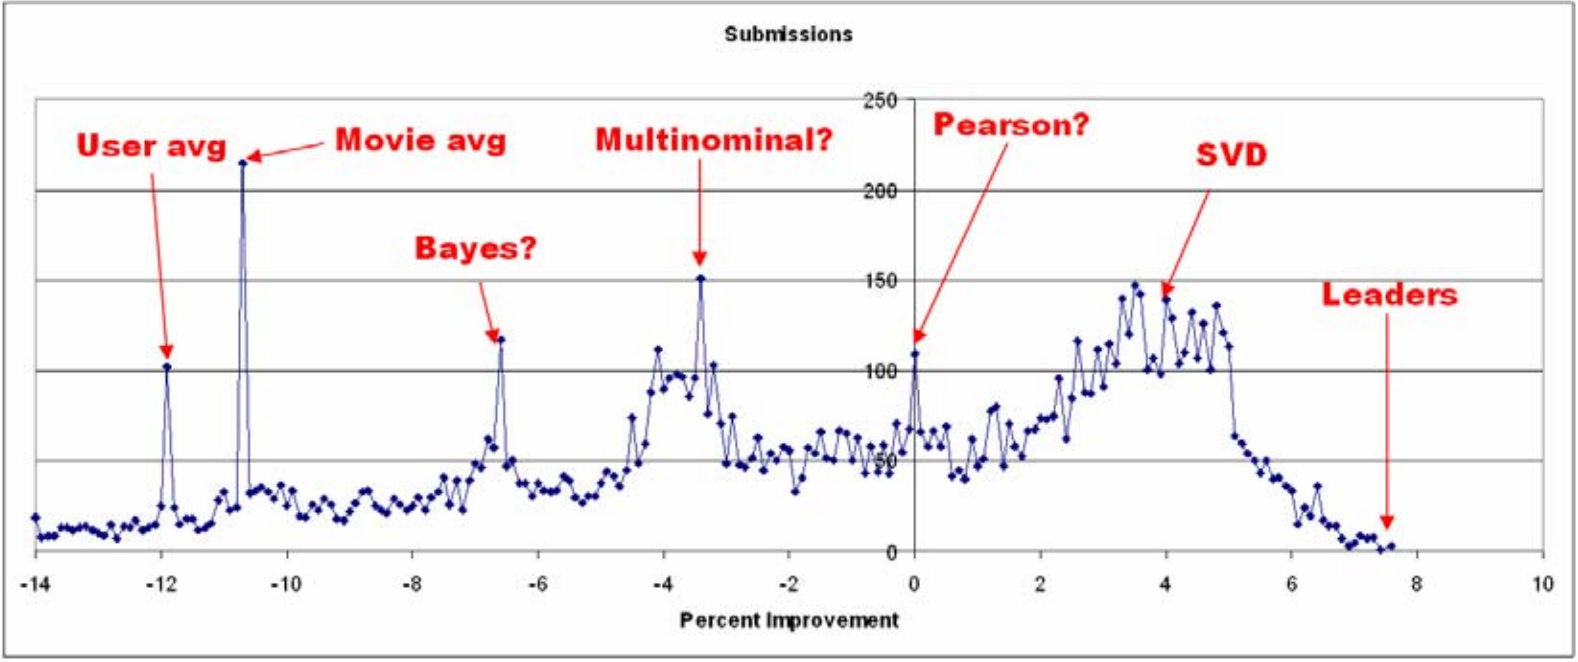
\includegraphics[width=5in]{image/sub-distr-nf.png}
\centering
\caption{Distribution of different submission amount, their score and the most used algorithms to produce the RMSE score. As we can see from the figure, one of the better performing algorithms are singular value decomposition (SVD). Approaches like using the average movie rating to suggest ratings and the average ratings for users, was often used, but did not produce a good recommendation (RMSE reduction from the Cinematch score by 10-12\%)}
\label{figure:sub-distr-nf}
\end{figure}

\subsubsection{Dataset statistics}
% http://en.wikipedia.org/wiki/Principal_components_analysis
% http://en.wikipedia.org/wiki/Singular_value_decomposition
% http://en.wikipedia.org/wiki/Latent_semantic_indexing
% http://www.timelydevelopment.com/demos/NetflixPrize.aspx

To better understand the dataset, some statistics about the dataset was produced.

\begin{figure}[H]
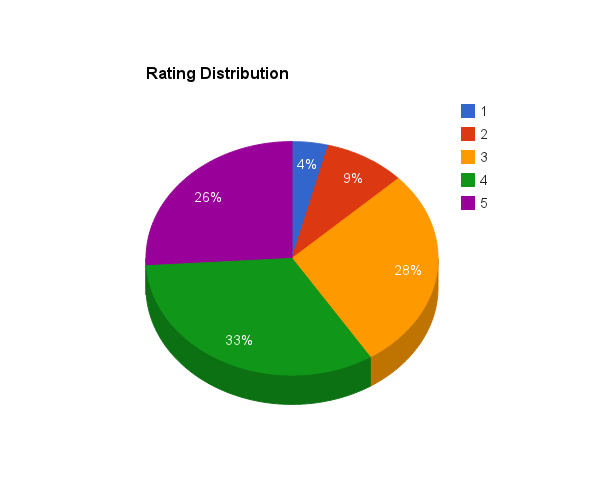
\includegraphics[width=5in]{image/ratingdistr.png}
\centering
\caption{Rating distribution}
\label{figure:ratingdistr}
\end{figure}

Rating distribution is shown in figure~\ref{figure:ratingdistr}. 1/3 of the ratings are 4, and rating 1 and 2 only makes up for 13\% of the rating distribution. 3 and 5 are quite similarly represented with 28\% and 26\% respectively. It can from this be assumed a greater prediction towards the higher ratings, and predictions towards lower ratings should not be done lightly.

\begin{figure}[H]
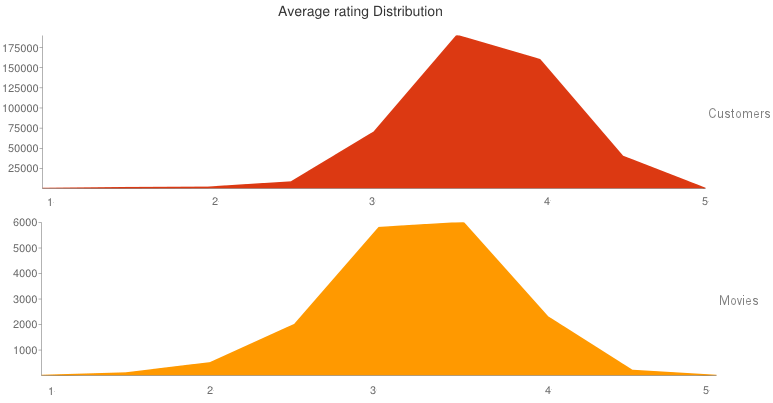
\includegraphics[width=5in]{image/avgratingdistr.png}
\centering
\caption{Average rating distribution}
\label{figure:avgratingdistr}
\end{figure}

\begin{figure}[H]
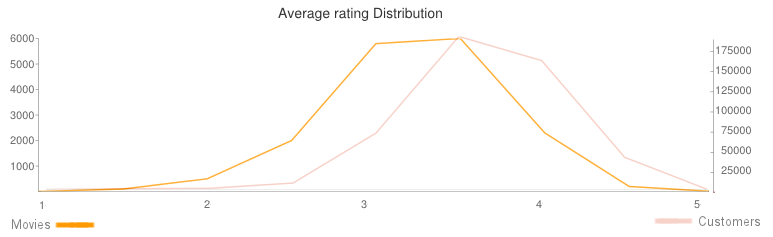
\includegraphics[width=5in]{image/avgratdistrover.png}
\centering
\caption{Average rating distribution}
\label{figure:avgratdistrover}
\end{figure}


Average rating distribution is shown in figure~\ref{figure:avgratingdistr}. The upper graph shows average rating distribution of the customers, while the bottom one shows the distribution per movie. Both graphs have quite similar form. Both customers and movies peak at a rating of 3,5, which is natural. The second second highest point is for the customers at 4 and movies at 3, which is interesting to see. TO ANALYSE MORE!


\begin{figure}[H]
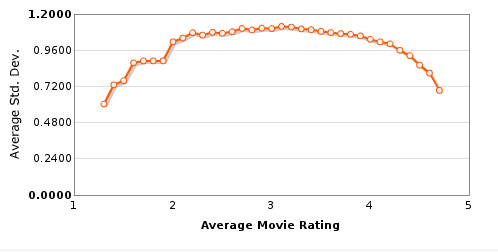
\includegraphics[width=5in]{image/avgmovierating.png}
\centering
\caption{Average movie rating distribution}
\label{figure:avgmovierating}
\end{figure}

Average movie rating distribution is shown in figure~\ref{figure:avgmovierating}. Here we see that for the edge ratings (rating 1 or 5) has the least standard deviation, so when a movie is highly rated it usually is rated high, and the same goes for low ratings, while for the middle ratings (2 to 4) we see that it variates more, and quite similarly. So the middle ratings are harder to classify, in other words, when a movie has a rating of 3, the average rating-shift is almost 1.1, so it must be expected that there is a bigger classification hit on these, so the problem will be to fin the right classification.





% End Netflix



% About Weka
\section{Weka}
%http://en.wikipedia.org/wiki/Weka_(machine_learning)

\begin{wrapfigure}{r}{.30\textwidth}
\vspace{-30pt}
\centering

\includegraphics[width = .25\textwidth]{image/Weka-logo.png}
\end{wrapfigure}


Weka is a machine learning software written in Java. It can be used to visualize data through analyzing it with different kinds of algorithms. The Explorer, a graphical user interface, makes it easy to work with and explore data from different angles. It is a free software under the General Public License \cite{GNU}. Weka can handle several data mining tasks, including, data preprocessing, clustering, classification, regression and feature selection. The input data has to be a single flat file or relation, each data point must be described by a fixes number of attributes. The dataset can be accessed trough a SQL database. Can link database tables into a single datatable, which can be used for processing using Weka.


\subsection{ARFF}
% http://www.cs.waikato.ac.nz/ml/weka/arff.html
Attribute Relationship File Format is the file type used to store data in a database. The structure is as follows:

\begin{lstlisting}[caption={ARFF Example},label={lst:arffEx},captionpos=b]
@relation 'flat-netflix'

@attribute assetId string
@attribute 14367 numeric
@attribute 6050 numeric
@attribute 14112 numeric

@data
1658496,?,?,4
684232,3,3,?
684231,4,?,?
1774519,1,?,?
\end{lstlisting}

Listing~\ref{lst:arffEx} is an example of how an ARFF file is structured. It startes with a header, containing "@relation", "@attribute"s and the "@data". This header defines the name of the relation, the attributes in the dataset and the data. The "@data"-header contains arrays, where each array has values for the corresponding "@attribute"s values. If a array has no value for a particular attribute it is denoted as a question mark (?).

\subsection{The Explorer}
% http://www.cs.waikato.ac.nz/~ml/weka/gui_explorer.html
% http://research.cs.queensu.ca/home/cisc333/tutorial/Weka.html
% http://wiki.pentaho.com/display/DATAMINING/Time+Series+Analysis+and+Forecasting+with+Weka
\begin{table}[H]
\centering
\begin{tabularx}{1.0\textwidth}{ l p{9.3cm} }
  \textbf{Components} & \textbf{Description} \\
  \hline \\ [-1.5ex]
  Preprocess & Here the user can import the data which is going to be analyzed. It is also possible to do some filtering on this data, this includes removing of values and transforming values. \\
  \hline \\ [-1.5ex]
  Classify & Here the user can apply classification and regression algorithms to the dataset. \\
  \hline \\ [-1.5ex]
  Associate & Here the user can have the association rule learners identify important relationships between attributes in the provided dataset. \\
  \hline \\ [-1.5ex]
  Cluster & Here the user can apply cluster algorithms to the dataset \\
  \hline \\ [-1.5ex]
  Select attributes & Here the user can identify the most predictive attributes in the dataset. \\
  \hline \\ [-1.5ex]
  Visualize & Here the user can get a visualization of the dataset, and of the different algorithms preformed on the dataset. \\
\end{tabularx}
\caption{Classification based on feature}
\label{table:nosql-calssifications}
\end{table}

\subsection{Machine-learning algorithms}
Weka can let the user utilize its many machine-learnings algorithms in an easy and convenient way. It opens for easy implementations of the algorithms though both just input of a file and get a result back, or though incorporating the algorithms in code.
% End Weka




% About Twitter
\section{Twitter}\label{sec:twitter}

\begin{wrapfigure}{r}{.30\textwidth}
\vspace{-30pt}
\centering

\includegraphics[width = .25\textwidth]{image/twitter-logo.png}
\end{wrapfigure}
Twitter is a free social media network based on microblogging. In microblogging, a user can post a paragraph of a certain number of characters or less to his/her timeline. The user can also follow other users. Whenever the users that a given user is following posts something, the user can see these posts in his/her feed. This is the basis for many of todays most popular social media networks, including Twitter.

\subsection{Terminology}
For more clarity, we define the terminology twitter uses. All words in \textbf{bold} are our own definitions for more easily describing how the various term relate to eachother.

\subsubsection{Tweet}
A tweet is a post containing max 140 characters. It can also refer to the verb ‘to tweet’, which means ‘to post a tweet’. \textbf{tweets} is an attribute of a user which returns a list of tweets that the users

  \textbf{user.tweets -> [<tweet>]}
\subsubsection{User}
A user is someone with a twitter account. A user can post tweets. By following other users, twitter generates a feed for the user containing the tweets of all the users they follow. They also have certain information retrieval tools available, such as filtering tweets by a tag name, specific user or search term.

\subsubsection{Tweeter}
A user who tweets a tweet that is referenced in the same context. For instance: The best tweets are tweeted by the most popular tweeters


\subsubsection{Follower}
A follower is someone who follows a user. The follower will see the users tweets in their feed. \textbf{followers} is an attribute of a user which returns the list of users that are following that user.

  \textbf{user.followers -> [<user>]}

\subsubsection{Followee}
A followee is someone who a user is following. The user will appear in the followees list of followers, and the followee will appear in the users list called ‘following’. We will refer to the list ‘following’ for a user as followees for clearer terminology. \textbf{followees} is an attribute of a user which returns the list of users that the user is following.

  \textbf{user.followees -> [<user>]}

\subsubsection{Hashtag}
Hashtags are topic labels that are placed on tweets. They are made by typing \#topicname anywhere in the tweet. By navigating to \#topicname, a user will see a feed of all tweets containing \#tagname. \textbf{hashtags} is a an attribute of a tweet which returns the list of hashtags the tweet contains.

  \textbf{tweet.hashtags -> [<hashtag>]}

\noindent
Hashtag also has the attribute tweets, which returns all tweets that have a certain hashtag. These hashtags are ordered by twitters algorithm which balances how recent the tweet is with the popularity of the tweeter.

  \textbf{hashtag.tweets -> [<tweet>]}

\subsubsection{Usertag}
Usertags are labels that are placed on tweets describing who the tweets are adressed to. They are made by typing @username anywhere in the tweet. This tweet will also show up in the feed of the user with name username. \textbf{usertags} is an attribute of a tweet which returns the list of users that the tweet is adressed to.

\textbf{tweet.usertags -> [<user>]}

\subsection{Legal Considerations}
Collect and use a data set from twitter, a company whose currency is information, must be done in a way that complies with their rules and terms of service. This section considers how an automated system can collect information from twitter and what an automated system can use it for.

\subsubsection{API Terms}
You may use the Twitter API and Twitter Content in connection with the products or services you provide (your "Service") to search, display, analyze, retrieve, view, and submit information to or on Twitter \cite{twitter-api-terms}. This means that data can be gathered within the limitations set by the API to gather a dataset and analyze it.

If you provide downloadable datasets of Twitter Content or an API that returns Twitter Content, you may only return IDs (including tweet IDs and user IDs) \cite{twitter-api-terms}. A system that utilizes the API to gather and analyze a dataset can be built and run legally as long as the dataset is not made available, or the dataset only contains IDs.

\subsubsection{General Terms of Service}
Crawling the Services is permissible if done in accordance with the provisions of the robots.txt \cite{twitter-robots-txt} file, however, scraping the Services without the prior consent of Twitter is expressly prohibited \cite{twitter-tos}. It is thus possible to crawl twitter as long as only the page is being indexed and it is done in accordance with robots.txt. Scraping the pages for tweets and other data can only be done with the prior consent of Twitter. Twitter has been contacted about whether or not data can be scraped for analysis in context of movie recommendations for a thesis, but has yet to reply.


\subsection{REST API}
Twitters HTTP/HTTPS based REST API allows the application using it to perform many of the core functionalities of Twitter. The fully reflects Twitter's content.

\subsubsection{Usage}
The API is divided into POST and GET requests. The POST requests makes changes to twitter. A POST request could be for posting a tweet, update a users profile etc. The GET requests retrieves data from twitter. A GET request could be used to retrieve followees or followers of a user, retrieve the tweets on the timeline of a user etc. The data is returned as JSON. \cite{twitter-rest-api}

\subsubsection{Authentication}
Twitters REST API uses an access token generated for the specific application in order to make a request. In addition, OAuth can be used if the session is on behalf of a specific user. Some requests such as posting a tweet can of course only be made on behalf of a user and thus requires OAuth. \cite{twitter-rest-api}

\subsubsection{Rate Limit}
The number of requests an application or a user can make is limited to a 15 minute window. Within this 15 minute window the each user can make 15 GET requests. This means that a user can retrieve the followees of 15 users withing the 15 minute window, but must wait until the 15 minutes have passed before retrieving more data. This means that large amounts of data can only be retrieved over long periods of time.

If only the application access token is used and not OAuth, the application as a whole can make 15 GET requests within the window. \cite{twitter-rate-limiting}

\subsection{Search API}
Twitters Search API is a REST API that is used for searching for tweets that match a search query.

\subsubsection{Usage}
The Search API uses only GET requests. Each GET request contains the search query as well as other parameters such as location to specify the search further. The API will return tweets that contain any of the words in the search query in any order. The tweets are returned as JSON.\cite{twitter-rest-api}

It is important to note that not all tweets are indexed in the Search API. Only a selected number of tweets, possibly within only a certain time frame are available. The tweets returned by the Search API are thus only a subset of all tweets.\cite{twitter-search-api-timeframe}

\subsubsection{Authentication}
To authenticate, the access token generated for the application can be used as well as OAuth. This is the same as the REST API. \cite{twitter-rest-api}

\subsubsection{Rate Limit}
The number of requests that can be made are limited to 180 requests per 15 minute window for each OAuth. If the Search API is accessed using only the application access token, these limitations apply application-wide for any number of users.\cite{twitter-rate-limiting}

\subsection{Stream API}
Twitters Stream API streams data from twitter as it is created to a client through a persistent HTTPS connection. It is ideal for gathering the most up-to-date tweets or gathering large amounts of data over long periods of time.

\subsubsection{Usage}
The client makes an initial GET request specifying the type of data it wants to receive. The request contains a list of up to 400 keywords. Any tweet that matches one or more of these keywords are considered part of the stream. The request can be directed to two endpoints: A public endpoints, which streams tweets from all users; or a user endpoint, which sterams tweets from a specific user.

After the initial request is made, a persistent HTTP connection is opened. Then, the tweets that match the keywords in the initial request are streamed. The tweets keep streaming until the connection closes.

\subsubsection{Authentication}
Authentication for using the Stream API is done with OAuth. There is no application wide identification such as in the REST API and the Search API.

\subsubsection{Limitations}
There is no rate limit in the Stream API. However, there are a few cases in which the streaming will stop. For instance, If the client fails to receive the streamed data and twitters buffer builds up too many tweets, the connection will be closed. Also, if the client opens too many streams with the same credentials, the oldest connection will be closed.

\subsection{Crawling and Scraping Twitter}
TODO: Add appendixes from scrapbook.
This section will examine how to crawl and scrape Twitters HTTPS Web Search. This will be examined by browsing twitter.com logged in as a user and examining it Google Chrome Developer Tools (GCDT)\cite{gcdt} as the site is being browsed and search requests are being made. The goal of this examination is to discover requests a webcrawler must be capable of making in order to search twitter and harvest tweets and users automatically and how a scraper can distinguish the dom elements that describe a tweet.


\subsubsection{Search Request}
Tweets can be found using an HTTPS search request with the search query in the format URLE \cite{w3-urle-ref}
Searching for <URLE search query> can be done with the HTTPS request shown in listing-\ref{listing:search-request}.
In the rest of the discussion, we'll be using the search query "The Dark Knight Rises 2012". The search request for this search query parsed to URLE is shown in listing-\ref{listing:search-request-batman-urle}

  \begin{lstlisting}[caption={URL of a twitter HTTPS search request for <URLE-search-query>},label={listing:search-request},captionpos=b]
  https://twitter.com/search?q=<URLE-search-query>&src=typd&f=realtime
  \end{lstlisting}

\begin{lstlisting}[caption={URL of a twitter HTTPS search request for "The Dark Knight Rises 2012" parsed to URLE},label={listing:search-request-batman-urle},captionpos=b]
  https://twitter.com/search?q=the%20dark%20knight%202012&src=typd&f=realtime
  \end{lstlisting}

Using the Google Chrome Developer Console \cite{gcdt} we can find the DOM elements on the search page that contains all the tweets that have been returned, using the select element tool. The HTML of this element is shown in listing-\ref{listing:tweet-container-html}. Within it, each tweet is contained in an HTML element like the one in listing-\ref{listing:tweet-element-html}

  \begin{lstlisting}[caption={HTML of the element containing all tweet elements},label={listing:tweet-container-html},captionpos=b]
  <ol class="stream-items js-navigable-stream" id="stream-items-id\">
  \end{lstlisting}

  \begin{lstlisting}[caption={HTML of a tweet element},label={listing:tweet-element-html},captionpos=b]
  <li class="js-stream-item stream-item stream-item expanding-stream-item" data-item-id="397530125715402752" id="stream-item-tweet-397530125715402752" data-item-type="tweet">...</li>
  \end{lstlisting}

Using jQuery \cite{jquery} and the Javascript Console in GCDT \cite{gcdt}, it is possible to determine how many tweets have been returned. This is done by defining javascript function that selects the tweets elements and returns the number of elements in this list in listing-\ref{listing:tweet-count-function}. The function can be assured to work by counting the number of tweets displayed on the search result page and making sure that it matches the number returned by the function.

  \begin{lstlisting}[caption={Creating a function in GCDT Javascript Console for counting the occurance of tweets on the twitter search result page},label={listing:tweet-count-function},captionpos=b]
  > number_of_tweets_in_search_results = function(){ return $("li[data-item-type='tweet']").size(); }
  > number_of_tweets_in_search_results();
  15
  \end{lstlisting}

\subsubsection{Scroll Search Results}
TODO: Add captions and references and use \$ for direct reference.
In order to obtain more search results it is necessary to scroll to the bottom of the page for the browser to make an XHR request to retrieve more tweets. As the scrolling is done, XHR requests can be monitored in the Network tab of GCDT. Consecutive xhr requests are sent as scrolling is done several times.

  \begin{lstlisting}[caption={TODO: Caption},label={},captionpos=b]
  Javascript Console:
  > number_of_tweets_in_search_results();
  15

  Network Console > XHR:
  Request URL:https://twitter.com/i/search/timeline?q=the%20dark%20knight%202012&src=typd&include_available_features=1&include_entities=1&last_note_ts=0&scroll_cursor=TWEET-360758159364734978-399762568459612160


  Javascript Console:
  > number_of_tweets_in_search_results();
  35

  Network Console > XHR:
  Request URL:https://twitter.com/i/search/timeline?q=the%20dark%20knight%202012&src=typd&include_available_features=1&include_entities=1&last_note_ts=0&oldest_unread_id=0&scroll_cursor=TWEET-338938038694584320-399762568459612160

  Javascript Console:
  > number_of_tweets_in_search_results();
  50

  Network Console > XHR:
  Request URL:https://twitter.com/i/search/timeline?q=the%20dark%20knight%202012&src=typd&include_available_features=1&include_entities=1&last_note_ts=0&oldest_unread_id=0&scroll_cursor=TWEET-316893896573607937-399762568459612160

  Javascript Console:
  > number_of_tweets_in_search_results();
  65
  \end{lstlisting}

As the requests are sent and processed, tweets are appended to the tweets element. All that is needed in order to keep receiving tweets is to keep sending requests of this pattern.
Examining the attributes of the XHR requests, they consists of the following variables and constants.

  \begin{lstlisting}[caption={TODO: Caption},label={},captionpos=b]
  constant src=typd
  constant include_available_features=1
  constant include_entities=1
  constant last_note_ts=0
  constant oldest_unread_id=0
  variable scroll_cursor=TWEET-<18 character number>-<18 character number>
  \end{lstlisting}

At this point a snapshot of the HTML page is taken [A3]. The only attribute that seems to variate with each request is scroll\_cursor attribute. This means that the piece of javascript code that is making the requests somehow has access to the information contained in this changing attribute. A DOM tree search for 'TWEET-' shows us that scroll\_cursor is contained by a div with the class stream-container under under the attribute 'data-scroll-cursor' and 'data-refresh-cursor'.

  \begin{lstlisting}[caption={TODO: Caption},label={},captionpos=b]
  <div class="stream-container" data-scroll-cursor="TWEET-311337362556846081-399762568459612160" data-refresh-cursor="TWEET-396773826303762432-399762568459612160">
  \end{lstlisting}

By making another scroll to the bottom of the page, a request with scroll-cursor information from one of these attributes is sent.
As is shown, the attribute data-scroll-cursor is responsible for what goes in the attribute scroll-cursor.

  \begin{lstlisting}[caption={TODO: Caption},label={},captionpos=b]
  Network Console > XHR:
  https://twitter.com/i/search/timeline?q=the%20dark%20knight%202012&src=typd&include_available_features=1&include_entities=1&last_note_ts=0&scroll_cursor=TWEET-311337362556846081-399762568459612160
  \end{lstlisting}

\subsubsection{Scraping Search Results}

Each tweet element in the search results contains DOM elements of importance that can be scraped. These DOM elements are shown in table-\ref{table:important-tweet-element-elements}.

\begin{table}[H]
\centering
\begin{tabularx}{5.3\textwidth}{ lp{7cm} lp{5cm} }
  \textbf{Element Name} & \textbf{Content}\\
  \cline{0-1}
  User Name & The name of the user who posted the tweet \\
  \cline{0-1}
  User ID & The ID of the user who posted the tweet \\
  \cline{0-1}
  Tweet Text & The text contained in the tweet
\end{tabularx}
\caption{Elements to be scraped from each tweet element that has been retrieved}
\label{table:important-tweet-element-elements}
\end{table}

\subsubsection{User Name}
The user name can be found in the header of the tweet. Using the GCDT Select, it can be extracted from the page as shown in blue in figure-\ref{figure:tweet-user-field}. It will be referred to as the user name element.

\begin{figure}[H]

\includegraphics[width=4in]{image/tweet-user-field.png}
\centering
\caption{User name element (shown in blue) in a tweet retrieved by twitter web search}
\label{figure:tweet-user-field}
\end{figure}

\begin{lstlisting}[caption={HTML of the user name element in a tweet},label={user-name-element-html},captionpos=b]
  <span class=\"username js-action-profile-name\"><s>@</s><b>BatmanMemorabil</b></span>
\end{lstlisting}

\noindent
Using jQuery, a function can be created to count the occurances of the class "username js-action-profile-name", as shown in \ref{user-name-element-count-jquery-function}. This function can then be used to compare the number of user name elements in the DOM tree to the number of tweets in the search result, as shown in listing-\ref{user-elements-matches-tweets}. Since they are equal, it is likely that the right class is being scraped for the user name element.

\begin{lstlisting}[caption={Creating a function in GCDT Javascript Console for counting the occurance of user name elements on the twitter search result page},label={user-name-element-count-jquery-function},captionpos=b]
  > number_of_tweet_user_name_element_occurances = function(){ return $("span.username.js-action-profile-name").size() }
\end{lstlisting}


\begin{lstlisting}[caption={Running functions in GCDT Javascript Console to show that the number of user name elements matches the number of tweets},label={user-elements-matches-tweets},captionpos=b]
  > number_of_tweet_user_name_element_occurances();
  119
  > number_of_tweets_in_search_results();
  119
\end{lstlisting}

\subsubsection{User ID}
The user ID can also be found in the header. It is contained in the attribute data-user-id. Using the GCDT Select, it can be scraped from the page. It will be referred to as the user id element. The HTML of this scraping is shown in listing-\ref{listing:user-id-element-html}

\begin{lstlisting}[caption={HTML of the user id element in a tweet},label={listing:user-id-element-html},captionpos=b]
  <a class="account-group js-account-group js-action-profile js-user-profile-link js-nav" href="/username" data-user-id="userid">...</a>
\end{lstlisting}

\noindent
Using jQuery, a function can be created to count the occurances of the class used to specify the user id element, as shown in \ref{user-id-element-count-jquery-function}. This function can then be used to compare the number of user id elements in the DOM tree to the number of tweets in the search result, as shown in listing-\ref{user-id-elements-matches-tweets}. Since they are equal, it is likely that the right class is being scraped for the user id element.

\begin{lstlisting}[caption={Creating a function in GCDT Javascript Console for counting the occurance of user id elements on the twitter search result page},label={user-id-element-count-jquery-function},captionpos=b]
  > number_of_tweet_user_id_element_occurances = function(){ return $("a.account-group.js-account-group.js-action-profile.js-user-profile-link.js-nav").size() }
\end{lstlisting}

\begin{lstlisting}[caption={Running functions in GCDT Javascript Console to show that the number of user id elements matches the number of tweets},label={user-id-elements-matches-tweets},captionpos=b]
  > number_of_tweet_user_id_element_occurances();
  21
  > number_of_tweets_in_search_results();
  21
\end{lstlisting}

\subsubsection{Tweet Text}
The tweet text can be found in the content of the tweet, as shown in blue in figure-\ref{figure:tweet-text-field}. Using the GCDT Select, it can be extracted from the page. It will be referred to as the tweet content element. The tweet content element contains several HTML elements from which the text can be scraped, as shown in listing-\ref{listing:tweet-content-element-html}.

  \begin{figure}[H]

\includegraphics[width=4in]{image/tweet-text-and-url-field.png}
\centering
\caption{Tweet content element (shown in blue) in a tweet retrieved by twitter web search}
\label{figure:tweet-text-field}
\end{figure}

\begin{lstlisting}[caption={HTML of the tweet content element in a tweet},label={listing:tweet-content-element-html},captionpos=b]
  <p class="js-tweet-text tweet-text">
    <strong>The Dark Knight</strong> Rises (DVD, <strong>2012</strong>)
    <a href="http://t.co/p8pr9wqC4k" rel="nofollow" dir="ltr" data-expanded-url="http://ift.tt/17i5F5V" class="twitter-timeline-link" target="_blank" title="http://ift.tt/17i5F5V">
      <span class="tco-ellipsis"></span>
      <span class="invisible">http://</span>
      <span class="js-display-url">ift.tt/17i5F5V</span>
      <span class="invisible"></span>
      <span class="tco-ellipsis">
        <span class="invisible">&nbsp;</span>
      </span>
    </a>
    <a href="/search?q=%23batman&amp;src=hash" data-query-source="hashtag_click" class="twitter-hashtag pretty-link js-nav" dir="ltr">
      <s>#</s><b>batman</b>
    </a>
  </p>
\end{lstlisting}

\noindent
Using jQuery, a function can be created to count the occurances of the class "js-tweet-text tweet-text", which most likely describes all tweet content elements. The function is shown in listing-\ref{listing:tweet-content-element-count-function}. By comparing this number with the number of tweets in the search results and making sure it is equal, we can be confident that this class is describing the correct DOM element. The comparison is shown in
listing-\ref{listing:tweet-content-element-count-comparison}

\begin{lstlisting}[caption={Creating a function in GCDT Javascript Console for counting the occurance of tweet content elements on the twitter search result page},label={listing:tweet-content-element-count-function},captionpos=b]
  > number_of_tweet_content_element_occurances = function(){ return $("p.js-tweet-text.tweet-text").size() }
\end{lstlisting}

\begin{lstlisting}[caption={Running functions in GCDT Javascript Console to show that the number of tweet content elements matches the number of tweets},label={listing:tweet-content-element-count-comparison},captionpos=b]
  > number_of_tweet_content_element_occurances();
  119
  > number_of_tweets_in_search_results();
  119
\end{lstlisting}

\noindent
First, in order to obtain the tweet text, everything that is not a link or contained in a link must be scraped from the tweet content element in listing-\ref{listing:tweet-content-element-html}. An example of the HTML of this scraping is shown in listing-\ref{listing:tweet-text-scrape}. Then, the tweet text is obtained by stripping the HTML of all tags.

\begin{lstlisting}[caption={The HTML of scraping everything from listing-\ref{listing:tweet-content-element-html} that is not a link},label={listing:tweet-text-scrape},captionpos=b]
  <strong>The Dark Knight</strong> Rises (DVD, <strong>2012</strong>)
\end{lstlisting}

% End Twitter



\section{Similar Systems}


\subsection{Recommender Systems}
In this section, we will discuss similar solutions and their relevance to our project.


\subsubsection{MovieLens}\label{subsec:MovieLens}
MovieLens is a movie recommendation system. A user creates an account and gets movie recommendations based on the user's own ratings through MovieLens' collaborative filtering algorithm. They use a item-item based algorithm. They take the 20 movies which are most similar to the target movie and see how these 20 movies where rated.\cite{grouplens}

The issue with using a strict item-item based correlation and the MovieLens recommendation system is that for a user with a low rating average, the user will very seldom get recommended movies with a top-average rating.


\subsubsection{MovieTweetings}\label{subsec:MovieTweetings}
MovieTweetings is an application for fetching movie ratings through the Twitter API from Twitter. The application search for ratings shared from IMDB, a movie information webpage, and stored. The user has the option of sharing the rating or not on Twitter, in the last case, the rating will not be caught by the MovieTweetings application.

With the use of a social media they wish to get a fresher dataset than using Netflix dataset, or MovieLens datasets~\ref{subsec:MovieLens}. At the time of writing the article they had more than 60 000 ratings, and about 500 new where added every day\cite{MovieTweetings}. The Twitter API is queried daily to update their database.

While querying the API for well structured tweets with ratings about movies are a good way to go when in search for a database with movie ratings, the data will be sparse. The data is not based on the users followers/followees, and will therefore not represent the social strength Twitter is capable of producing. A direct access to IMDB, rather than going through Twitter to get the rating information also seems like a simpler and more result-producing idea.


\subsubsection{Twittomender}
Twittomender is a followee recommender for Twitter. Twitter uses a friend's friend approach for recommending new Twitter-friends. This does not necessarily produce the most relevant recommendations for a user. Twittomender takes a collaborative approach to the problem. Tweets of a user are used and compare with other users tweets to to find similarities and recommend new Twitter-friendships\cite{twittomender}.

7 recommendation strategies, they are shown in table~\ref{table:to-strategies}.

\begin{table}[H]
\centering
\begin{tabular}{ l l }
  \textbf{Type} &  \textbf{Strategy} \\
  \hline \\ [-1.5ex]
  Content-based &  \pbox{20cm}{ (1) Users own tweets \\
                                (2) Followee’s tweets \\
                                (3) Follower’s tweets \\
                                (4) All tweets} \\
  \hline \\ [-1.5ex]
  Collaborative-based & \pbox{20cm}{  (5) Followee’s Ids \\
                                      (6) Follower’s Ids \\
                                      (7) All Ids }\\
  \hline \\ [-1.5ex]
\end{tabular}
\caption{The 7 recommendation strategies used by Twittomender}
\label{table:to-strategies}
\end{table}

The user interacts with the system through providing the system with their username on Twitter, the system produces a profile of the user based on tweets, and determines a score against other users based on most frequent terms amongst the users tweets. Each of the strategies are used from table~\ref{table:to-strategies} and top 20 from each are merged to a list where the most frequent users are returned as recommended users to explore for the user.

After testing on 1000 users the best performing strategy was a collaborative-based approach, users and follower connection.

What we can take from this is the strength of a user's followees.


\subsection{What the top Netflix-Prize contestants did}\label{subsec:thewinners}
\subsubsection{BellKor's Pragmatic Chaos}
BellKor's Pragmatic Chaos, the prize winners of the Netflix-Prize competition, was a group of scientists from AT\&T Labs, Yahoo!, Pragmatic Theory and Commendo Research \& Consulting. They achieved a RMSE of 0.8567, which was 10.06\% better than Netflix's own Cinematch score.

Models for the rating data is learned by fitting previously observed ratings, but since the model is to be used to predict feature ratings, overfitting the data. This achieved by regularizing the learned parameters. A regularization constant is used, and is set to L2 by default. This and other constant such as, step size and number of iterations are set manually through greedy manners. Where the algorithm is ran multiple times and constant value with best score is used. \cite{BellKor-CF-TD}

The winning algorithm was put together based on multiple different modeling techniques. Some of these modeling techniques are described below. \\\\


\textbf{Time of week rating}  The team saw that a user-rating done in the weekends had a tendency to have a higher value than a rating done on a Monday. This also applies for multiple ratings done the same day, higher ratings does not necessarily imply that the movie is much better than a movie rated lower another day, the user might just be in a good mood.

\textbf{Close User ratings}  Ratings done close to one another done by the same user implied that the user was rating based on the user's recollection of the rated movies, and not that the user just saw that movie, these ratings had to be handled in its own manner. This was because of the effect the faulty or old memories had on these ratings. The all time favorites/negatives are also usually in this bulk. While the movies which did not make much of an impression are forgotten. This helps us explain figure~\ref{figure:avgmovierating}, where we saw that movies with the edge ratings (1 or 5) had a lower rating distribution.

\textbf{Baseline predictors}  Some users has the tendency to rate on an overall average higher than other users.

\textbf{Movie like-ability}  Movies can go in and out of popularity. This change usually happens over a extended period.

\textbf{Frequency term}  The number of ratings a users gives on a specific day can help explains data-variability during that day.

\textbf{Matrix factorization with Temporal Dynamics (SVD)}  Single value decomposition use two sets pf static movie factors. Set one is used in all the models of the factors. Set two uses the movies rated by the user, normalizes the sum, and uses this as a user factor.

\textbf{Neighborhood model with Temporal Dynamics}  Most common approach to collaborative filtering. They used a item-item model based on global optimization. To predict rating of a new item based of rating an old item two sets of weights where used. One where the values of the ratings where accounted for, and one disregarding rating values.
A situation where a user rates an old item and a new item close to each other both in time and rating, is a better indicator that these items can be related to each other, than if two items are rated similarly, but with a greater timespan between each other.Therefore a decaying relationship is introduced between items. This decreased RMSE from 0.9002 to 0.8870.\cite{BellKor-CF-TD}

\textbf{Clustering}  In a cluster the average value is the predictor for the user/movie pairs in the cluster. Where the movie-set and user-set are divided randomly into 128 bins, and created $128*128=16384$ clusters. This was their only usage of clustering, they found that it had no measurable impact on the accuracy of the final blend\cite{pragmatictheory-sol}.

\textbf{Anchoring}  There is a order of when to watch some movies. For instance, some squeals are usually watched in the order they where made, and should be predicted that way. \\\\


Interestingly, the bias model with tanking in the factor that users change rating-scale over time, resulted in a RMSE of 0.9555, which is almost as good as the Cinematch Netflix was already using. The learning with the different modeling techniques is done by a stochastic gradient descent algorithm running for 30 iterations. This is the only time they use an automatic parameter tuner. \cite{BellKor-2008-sol}

The "BellKor's Pragmatic Chaos"-team used a lot of different models and did a lot of tweaking to get to the top. Some interesting findings to take from this is the importance of diversity and how central the timestamp of a rating can be.

\subsubsection{The Ensemble}
% http://www.the-ensemble.com/

A merger of the teams "Grand Prize Team" and "Opera Solutions and Vandelay United". They also managed to get a RMSE of 0.8567, and therefore a 10.09\% improvement as well. But lost since the "BellKor's Pragmatic Chaos"-team managed to submit their results 20 minutes earlier than "The Ensemble"-team.

The two merged teams, which made "The Ensemble" consisted of multiple smaller teams. They had all competed in the Netflix-Prize challenge, and had to put their heads and code together to get to the result they got to.

"The Ensemble"-team used a huge variation of models, just as the "BellKor's Pragmatic Chaos"-team.

After the competition was done "The Ensemble" tested a merger of their system with the "BellKor's Pragmatic Chaos"-system. The test RMSE of a 50/50 blend was 0.855476, which is a 10.19\% improvement. This is 0.10\% better then the teams managed to produce by themselves.

\subsubsection{Conclusion}
After looking at the two top contestants from the competition a pattern is starting to form. Diversity is key to be able to predict user-ratings at a top level.

While both the teams managed to produce a 10\% improvement over the original netflix algorithm, it was never taken into use\cite{nfbeyond5}. Even though SVD and and RBM lowers the RMSE to 0.88 alone, are they not as applicable as wanted. The actual rating amount is 50 times bigger than the training set, and for SVD to give an accurate value, it has to be recalculated for each new rating, which is not applicable in a world where live recommendation is expected\cite{nfbeyond5}.


\subsection{Recommender Algorithms}
\subsubsection{Probabilistic Neighborhood Selection}
A often used approach when recommending items is a neighborhood-based collaborative filtering. This approach often has the issue that it over-specializes and makes concentrated biases when recommending. When trying to estimate an unknown value, the nearest neighbors tend to produce a recommendation list with known items. The taste of the user is often multidimensional when it comes to movies, and these can be unknown to the k nearest neighbors to the user\cite{umana}. This can be handled with a probabilistic approach when selecting neighbors\cite{probcobfilter}. The approach does not estimate an unknown value based on the weighted averages of the k nearest neighbors, but rather on k probabilistically selected neighbors\cite{optaplanner}. Another way of handling this issue is suggesting the least similar neighbors and their dislikes\cite{furthestneighbor}. This approach was proved to be less accurate when calculating the RMSE\cite{probcobfilter}, and will therefore not be explored further.

KNN is linear in the size of the training set, and therefore an efficient classification algorithm\cite{introtoIR}. And different implementations of it managed to produce RMSE scores from 0.91 to 1.002~\cite{knnnetflixstand, knnoldies, knnimpl, knncolbgroup}


\subsubsection{Matrix Factorization}\label{subsubsec:matrixfac}
There are several matrix factorization algorithms. Amongst them single value decomposition (SVD) and alternating least squares (ALS) are valid candidates. As we saw from Bellkor's solution~\ref{subsec:thewinners} single value decomposition was used, and was a good addition to their blend. The issue with this algorithm is that it is rather computationally expensive and re-computation is needed to be done when new ratings are added, and therefore not very applicable to a live recommendation system.

ALS is a simpler and a very parallelizable matrix factorization algorithm, more so than SVD, but with many of the benefits that matrix factorization brings\cite{predusingmatrix}. This makes it an interesting algorithm to look at.

This algorithm can be used to populate sparse matrices, just like the one from Netflix where the matrix is made up from users and movies. A rating matrix, $R$, is produced based on the use of two much smaller matrices. A number of "features" are set for each of the two smaller matrices $U$ and $M$, one for the users and one for the movies. The idea is to get $U^\top M$ as close to the real $R$. $U$ and $M$ are computed in two steps. This is easily parallelizable since solving for $U$ is independent of the other users, therefore the columns of $U$ can be computed in parallel. The information is gathered, and $M$ is updated, communication between movies is not necessary\cite{myrrix}. With this algorithm a 0.9278 was produced, which is a 2\% improvement over Cinematch~\cite{predusingmatrix}. Runtime to produce this score was 2 hours on a high-end system~\cite{alsMPI}.


\subsection{Conclusion}
There are two basic problems when analyzing very large datasets: Writing the code correctly and the performance (i.e. speed at which it runs). As we saw from \ref{subsubsec:matrixfac}, matrix factorization was one of the algorithms which preformed the best on the Netflix dataset. This is also shown in figure~\ref{figure:sub-distr-nf}. But the issue with it is if we want new ratings to be included in the recommendation system, then we need to recompute all recommendations, which is not ideally for a live recommendation system, where recommendation should include as much information as possible to be accurate.

The ALS~\ref{subsubsec:matrixfac} proved to be a very parallelizable algorithm, and a potential good alternative to SVD when doing live recommendation. But this requires a lot of computational power to make it live updating and will not be feasible to run on a low-end personal computer when wanting live results. But could prove to be a potential algorithm to use if one where to scale up to a high-end system.

The probabilistic neighborhood selection is a form of K-NN has a good runtime and produced a respectable RMSE. This is a well know approach to collaborative filtering, and there is a lot of documentations on different ways of selecting neighbors and implementation. This seems like the way to go as a start to produce recommendations on bigger datasets.
% end similar systems



\section{Development language and technologies}

\subsection{Database}
In order to easily retrieve data from the netflix prize dataset and store and retrieve data from twitter, it is useful to consider various kinds persistent storage or databases. There are three categories of options: Traditional file systems, SQL and NoSQL. Since traditional file systems are not designed for dynamically storing and retrieving data based on the structure of the data, they are not considered. The two options remaining are SQL and NoSQL which will be discussed and evaluated in the following sections.

\subsubsection*{NoSQL}
% http://en.wikipedia.org/wiki/NoSQL
NoSQL databases can be defined as: being non-relational. In many cases they are also: Open-source, distributed and horizontally scalable\cite{nosql}. NoSQL is meant for storing large amounts of data\cite{bigdata}, where all the data does not share the same attributes or schema. They are focusing on eventually consistency (BASE) instead of the more traditional consistent atomic transactions (ACID) \cite{pritchett}. The different kinds of NoSQL databases have different ways of classifying the database, some of the more used ones are: key-value, column, document, graph and relational.

\begin{table}[H]
\centering
\begin{adjustwidth}{-2cm}{}
\begin{tabularx}{1.3\textwidth}{  l l l l l l }
  \textbf{Data Model} & \textbf{Performance} & \textbf{Scalability} & \textbf{Flexibility} & \textbf{Complexity} & \textbf{Functionality}\\
  \hline \\ [-1.5ex]
  Key-value & high      & high              & high      & none      & variable (none)\\
  \hline \\ [-1.5ex]
  Column    & high      & high              & moderate  & low       & minimal \\
  \hline \\ [-1.5ex]
  Document  & high      & variable (high)   & high      & low       & variable (low)\\
  \hline \\ [-1.5ex]
  Graph     & variable  & variable          & high      & high      & graph theory \\
  \hline \\ [-1.5ex]
  Relational & variable & variable          & low       & moderate  & relational algebra\\
\end{tabularx}
\end{adjustwidth}
\caption{Differences in features of NoSQL Database Types}
\label{table:nosql-calssifications}
\end{table}
% http://www.slideshare.net/bscofield/nosql-death-to-relational-databases
As we can see from table~\ref{table:nosql-calssifications} performance, scalability and flexibility are usually rated as high in all the categories.

TODO: Move this to conclusion section
Relational algebra in the database will not be needed for the project to succeed so that category can be disregarded. High flexibility in the database would also be a feature sought after when going for NoSQL, so the column storage can also be eliminated from the equation. TODO: MAYBE SOMETHING MORE HERE lol the tree left are described well here : http://en.wikipedia.org/wiki/NoSQL
% http://en.wikipedia.org/wiki/Comparison_of_structured_storage_software
% http://www.mongodb.org/
\cite{nosql-databases, nosql-article}


\subsubsection*{SQL}
SQL databases are the most common way of storing structured data. The data is stored in columns and tables and is schema defined. This means that the attributes of the different datatypes are already defined and must be set whenever a datapoint is added to the database, even if it is NULL. The database can make relations between the tables id necessary, hence the name relational databases.
Performing queries is the way users and applications modify and read a SQL database. They are simple operations such as SELECT, UPDATE and DELETE written in the SQL query language. On a higher level of abstraction are transactions. Transactions are more or less a collection of queries. SQL Databases follow the ACID(atomicity, consistency, isolation, durability) principles for transactions. This means that the state of the database will never appear partially modified by a transaction to a new transaction that is being executed. Consistency of transactions are great for ensuring consistency across the data, but come at a performance cost.
\cite{ramakrishnan2003database}

\subsubsection{Database Alternatives}
Recommender systems are in nature performance heavy. They are also statistical which makes them fault tolerant. For this reason we have valued performance over consistency. The dataset is likely to have nested structure as it will combine two different types of data. Being able to append and combine data based on the structure of the content thus has value.
For these reasons the alternatives centered around NoSQL document stores, which are fast and have supports operations based on the structure of the document.
MySQL, which is the faster of the SQL alternatives, was also considered.

\subsubsection*{MongoDB}
MongoDB is a large scale, high availability, robust system. It is a NoSQL document store. Instead of storing the data in tables as in SQL, the data is stored in a BSON document. BSON stands for Binary JSON and is essentially a JSON document that is stored in binary instead of ASCII. A JSON document is a nested hash which can hold any number of attributes without depending on the other documents in the store. It is thus schemaless. Even though it is schemaless, MongoDB still possesses the some of the great properties from SQL databases, such as indexes, dynamic queries and updates.

MongoDB is implemented in C. It also has sharding which allows the database to scale horizontally. Custom queries and map-reduce queries can be written in JavaScript which has fast interpreters. This makes mongoDB an efficient and high speed data base for storing, modifying and fetching data with a nested document structure \cite{mongodb-intro}. In addition it has bindings to many different languages, which is a great advantage if some of the modules that need to access the database needs to be written in a language other than what it originally was written in.


\subsubsection*{CouchDB}
CouchDB is similar to MongoDB in the sense that it is a NoSQL Document store. It also has the same query capabilities as mongo and also uses JavaScript as a query language. In addition, CouchDB has a HTTP REST API which allows any web application to access it easily. CouchDB has a lot of built in features which makes web development with CouchDB easy. One of the greatest advantages is the intuitive web-based admin user-interface that is provided.
CouchDB does not support sharding which makes it less horizontally scalable. An alternative to achieve this is to use CouchBase, which is the distributed version of CouchDB. CouchDB is implemented in erlang. While erlang is faster than it used to be, it is certainly slower than a similar system written in pure C. In addition, CouchDB stores a copy of every single document every time it is modified. This makes CouchDB grow in size with time.
\cite{couchdb-about, couchdb-technical}


\subsubsection*{MySQL}
MySQL is one of the most popular database in the world of open databases. This is because of its high performance, reliability and ease of use. It should therefore be considered for the question of which database system to use. MySQL is an SQL based relational database, as opposed to the two NoSQL databases. It has bindings to most languages. It provides a much more advanced high level query language than a typical NoSQL document store. This is great for easily making complex queries during development, which is somewhat more tricky in NoSQL and JavaScript. However it is somewhat slower because of the interpretation of this high level language. The SQL database schema makes it more difficult to change the format of the data. MySQL also does not support JSON which is one of the most common standards for data retrieved from the web. This creates extra work with parsing JSON to the schema or invoking a mapper that has been created for this purpose.
\cite{mysql-about}


\subsubsection{Conclusion}
Even though MySQL has several of the properties needed for a recommendation system, it lacks the speed of a NoSQL store, which is a huge advantage. The complex join capabilities are not strictly necessary and can be replicated in JS in any of the two NoSQL document stores.

CouchDB has some unique merits. The simple web UI and HTTP REST API are great for development and compatability with web applications. However, compared to mongoDB it scores low on performance both as a standalone database, and in the sense that it can not be sharded to increase performance horizontally if necessary. It also takes up more space than necessary and grows in size for every single modification, which is an unfortunate property for a database that should handle a large fault tolerant dataset.

For these reasons mongoDB was chosen as the most appropriate alternative.


\subsection{Programming languages}
The main focus of our project is to harvest large amounts of data from the web, store it quickly in a database and do large computations on this data quickly. Because the design and implementation is likely to go through many iterations, it is important that the language chosen is most of all easy to modify. Performance of the language is also a valuable property.

\subsubsection{Ruby}
Ruby is a dynamic, interpreted, open source programming language with a focus on simplicity and productivity. Even though it is some times difficult to interpret ruby because there are always a large number of different ways to achieve the same functionarlity, ruby has an elegant syntax that is natural to read and easy to write. This is due to the fact that everything in Ruby is an object. Essential parts of Ruby can be removed or redefined, at will. Existing parts can be added upon. Ruby tries not to restrict the coder. This makes Ruby very flexible. \cite{ruby-about}

Ruby has one of the largest and most well crafted packaging systems of any language today. Packages in ruby are referred to as gems. RubyGems.org hosts more than 66000 gems to date. Gems can easily be created with the gem development tools that come with ruby. Gems also have very advanced yet simple requirement specification through Gemfiles. The name of required gems and ranges of working versions are specified in the Gemfile. All required gems can then be fetched with a single command. Creating a new gem or publishing a gem are also single commands. This makes managing dependencies and reusing code in ruby a breeze.\cite{rubygems}

Ruby is probably one of the most prevalent languages for modern web development. PHP is most likely still the most widely used, but ruby based web projects tend to be more managable due to the higher level frameworks and packages that are available.

\subsubsection{Python}
Python is a dynamic interpreted open source programming language. It is similar ruby in many ways. It has natural short typed syntax that is easy to read and write. For being an interpreted language, python is pretty fast. Python does not have an intuitive way of modifying existing parts of the language.\cite{python-about}

Python has a packaging system that is easy to use called Python Package Index, PIP for short. PIP hosts more than 37500 packages to date and has a very simple requirement specification and installation that only requires a few commands. This makes managing dependencies with python very easy.\cite{pip}

Python is widely used for a variety of cases. In particular science and web development. It also has some mature information retrieval libraries.

\subsubsection{Conclusion}
Python and Ruby are both great programming languages that fulfill the needs for writing modifiable code that can harvest and make predictions on data.

Python is slightly faster and has more mature information retrieval libraries. Ruby has more general packages available for reuse and is somewhat more modifiable.

The speed of python does not matter in the context of a web bottle neck. The algorithms in the information retrieval libraries must most likely be reimplemented to work with a database as these tend to do all predictions in memory. Because of this and because the authors have more experience with ruby, ruby was chosen over python.


\section{Result Testing}
Root-mean-square error (RMSE)~\ref{subsubsec:rmse} is a way of testing estimated value against the actual value. This is how they measured the correctness of the submitted solutions in the Netflix prize competition. To explore the correctness and improvement of the solution, this seems like a good way to go. The recommendation system will be ran on both the netflix-dataset alone and on the netflix-dataset merged with the twitter-data.

A reduction in the RMSE value will then indicate an improvement, and indicate the gain from the collaboration of movie data and social media data.

\section{Evaluation (maybe)}
TODO:
To sum up what we saw after the prestudy

\chapter{Requirements}

\minitoc

How requirements  were  captured;
  discussion  of  major requirements
(referring  to  Appendix  A for details).

I “Requirement”-kapittelet forklar hvordan du satt opp kravene.
Men ikke ha med en fullstendig oversikt over kravene her!

\clearpage


\section{Functional Requirements}

\begin{itemize}
  \item Harvest Twitter
  \item Find movies in user-tweets
  \item Find movie-tweets from tweeters the user is following
  \item
  \item Supplement netflix-dataset with Twitter-findings
  \item Test recommendation ability with improved netflix-dataset
  \item Generate reports
  \item
\end{itemize}


\section{Non Functional Requirements}

\begin{itemize}
  \item System should improve the RMSE
\end{itemize}


\section{Requirements Evaluation}


\section{Prioritized Requirements}


% !TEX root = ../report.tex

\chapter{Design}

\minitoc
This chapter the architecture and components in the architecture, how they were designed, and how they fulfill the requirements of the project.


\clearpage


\section{Definitions}


\section{Architecture}
The architecture of the project is based on The 4+1 View
Model of Software Architecture \cite{Kruchten}. The views are used reflect the structural aspects, temporal aspects, technological development aspects and physical aspects of the project.

The architecture uses a custom simplified version of the 4+1 notation that better fits the descriptive needs for the project.


\subsection{Logical View}
The logical view describes the components of the architecture and how they relate to one another in terms of containment, inheritance and usage. The logical view can be found in figure-\ref{figure:logical-view} and the notation for the logical view in figure-\ref{figure:logical-view-notation}

\begin{figure}[H]
\centerline{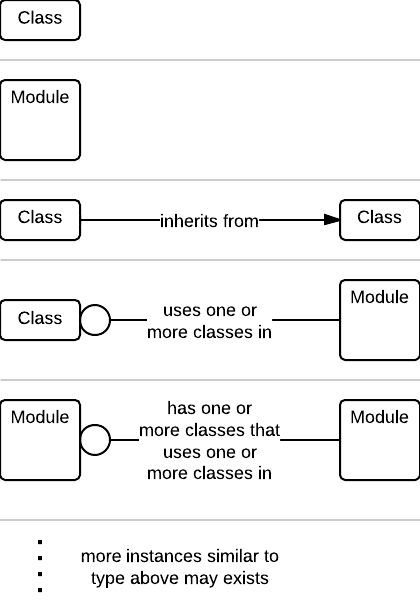
\includegraphics[width=2.5in]{image/architecture-logical-view-notation.png}}
\caption{Notation for the logical view.}
\label{figure:logical-view-notation}
\end{figure}

\begin{center}
\begin{figure}[H]
\centerline{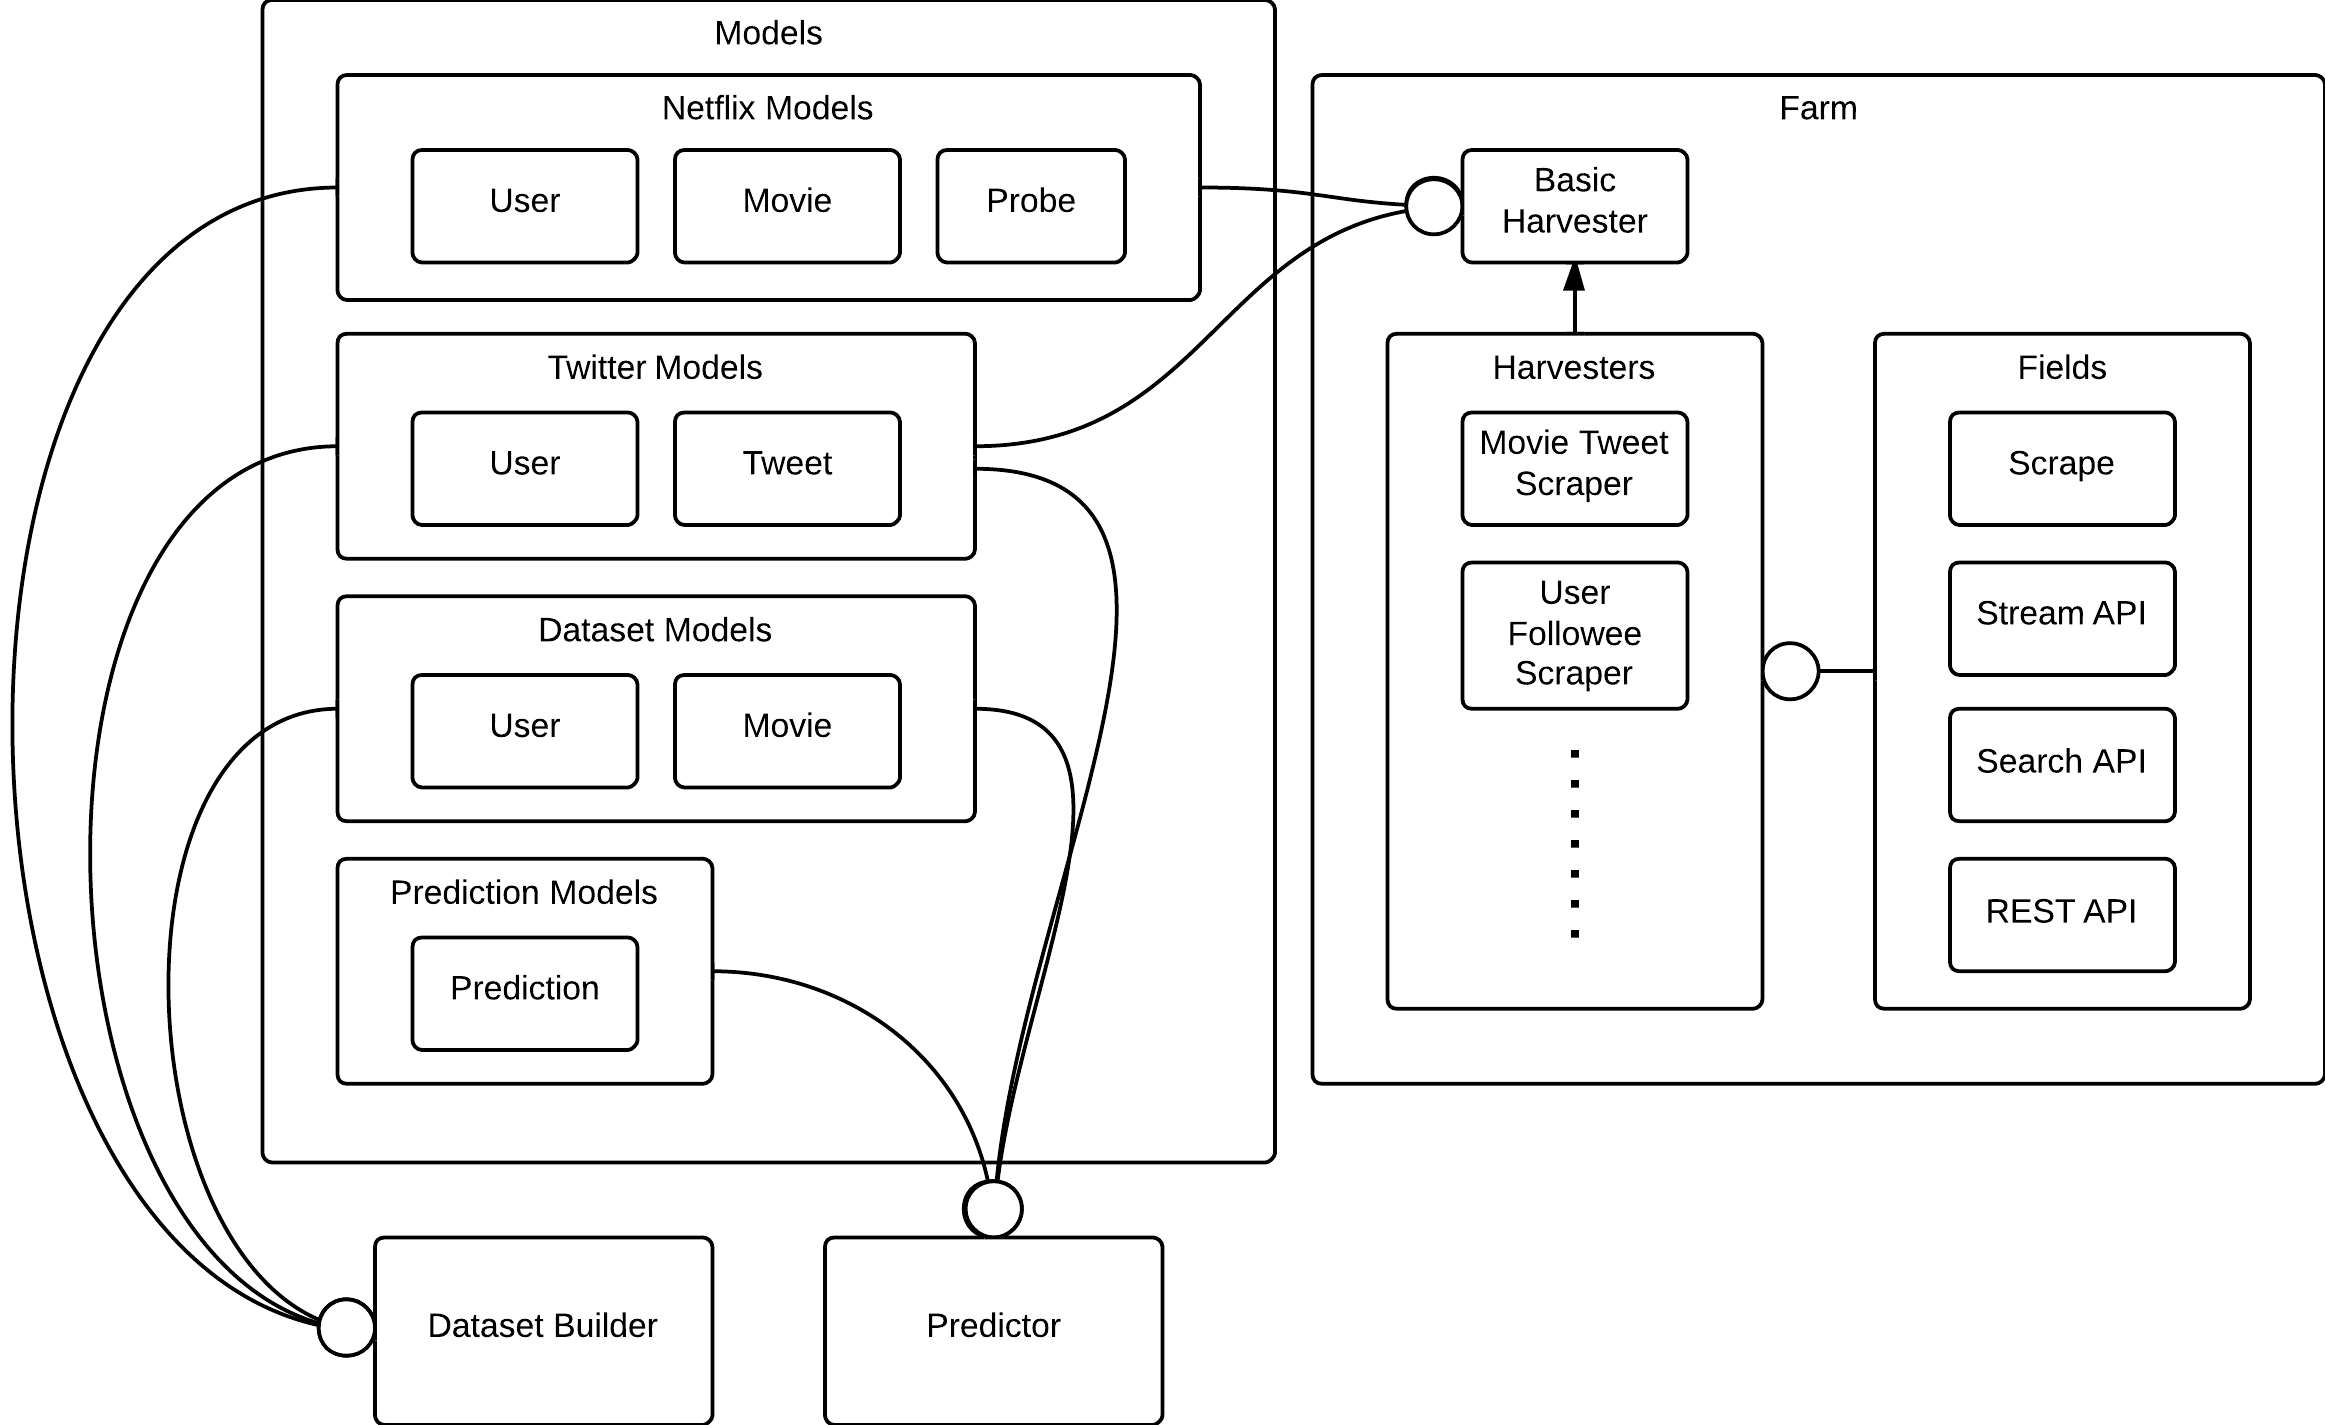
\includegraphics[width=7in]{image/architecture-logical-view.png}}
\caption{Logical view of the project. See figure-\ref{figure:logical-view-notation} for notation.}
\label{figure:logical-view}
\end{figure}
\end{center}

\subsubsection{Models}
Models is the module responsible for holding the different datamodels that are used in the project. It is found in the upper left part of the logical view in figure-\ref{figure:logical-view}. All classes in this module are mapped to and reflect the database.

The Netflix Models model the netflix prize dataset. Each user has a list of movie ratings and each movie has a list of user ratings. The probe is a list of movies with empty user ratings that need to be predicted.

The Twitter Models reflect the data harvested from Twitter. The schema of these models are variable as it depends on what type of data is harvested. A tweet typically contains a text and refers to a user. A user typically has a name and a user ID and may refer to tweets. As an example, it may also contain a list of followees or followers.

The Dataset Models reflects the Netflix Models after they have been mapped to fused with Twitter Models by the Dataset Builder.

The Prediction Models model what the ratings that the Predictor predicts using the Datast Models and the Probe in Netflix Models.

\subsubsection{Farm}
Farm is the module responsible for accessing and gathering data from Twitter.

The fields access Twitters data. Most fields implement one of Twitters existing APIs. There is also a Scrape field for accessing Twitters web search and scraping the results. It is important to note that Twitter does not allow this without explicit consent. Each field is implemented in such a way that it delivers a subset of the Twitter data types that are outlined in the functional requirements in section~\ref{section:functional-requirements}. The fields combined delivers all the Twitter data types in the requirements. The reason for dividing the access over several fields is that some of the fields are unsuitable for gathering certain Twitter data types.

The harvesters uses the fields to gather and store Twitter data that matches a model that already exists in either the netflix model or the twitter model. It is used for finding say tweets for a movie using the scraper field, followees for a user using the rest field or users for a movie using the stream field.

\subsubsection{Dataset Builder}
The dataset builder is responsible for building a dataset that reflects the netflix dataset using the data gathered from twitter by the harvesters. This new dataset is stored in dataset model.

\subsubsection{Predictor}
The predictor is responsible for predicting movie ratings for a collection of users. The predictor does so by for a test set and comparing it to several entries in a dataset. The test set is usually the probe in the netflix models. The dataset that the test set is compared to, is either the dataset model or the netflix model. The predictor also gradually calculates RMSE as it is predicting ratings.

\subsection{Process View}
The process view describes the actions that the components of the architecture engage in over time and how there actions relate to other components. See figure-\ref{figure:process-view}

\begin{figure}[H]
\centerline{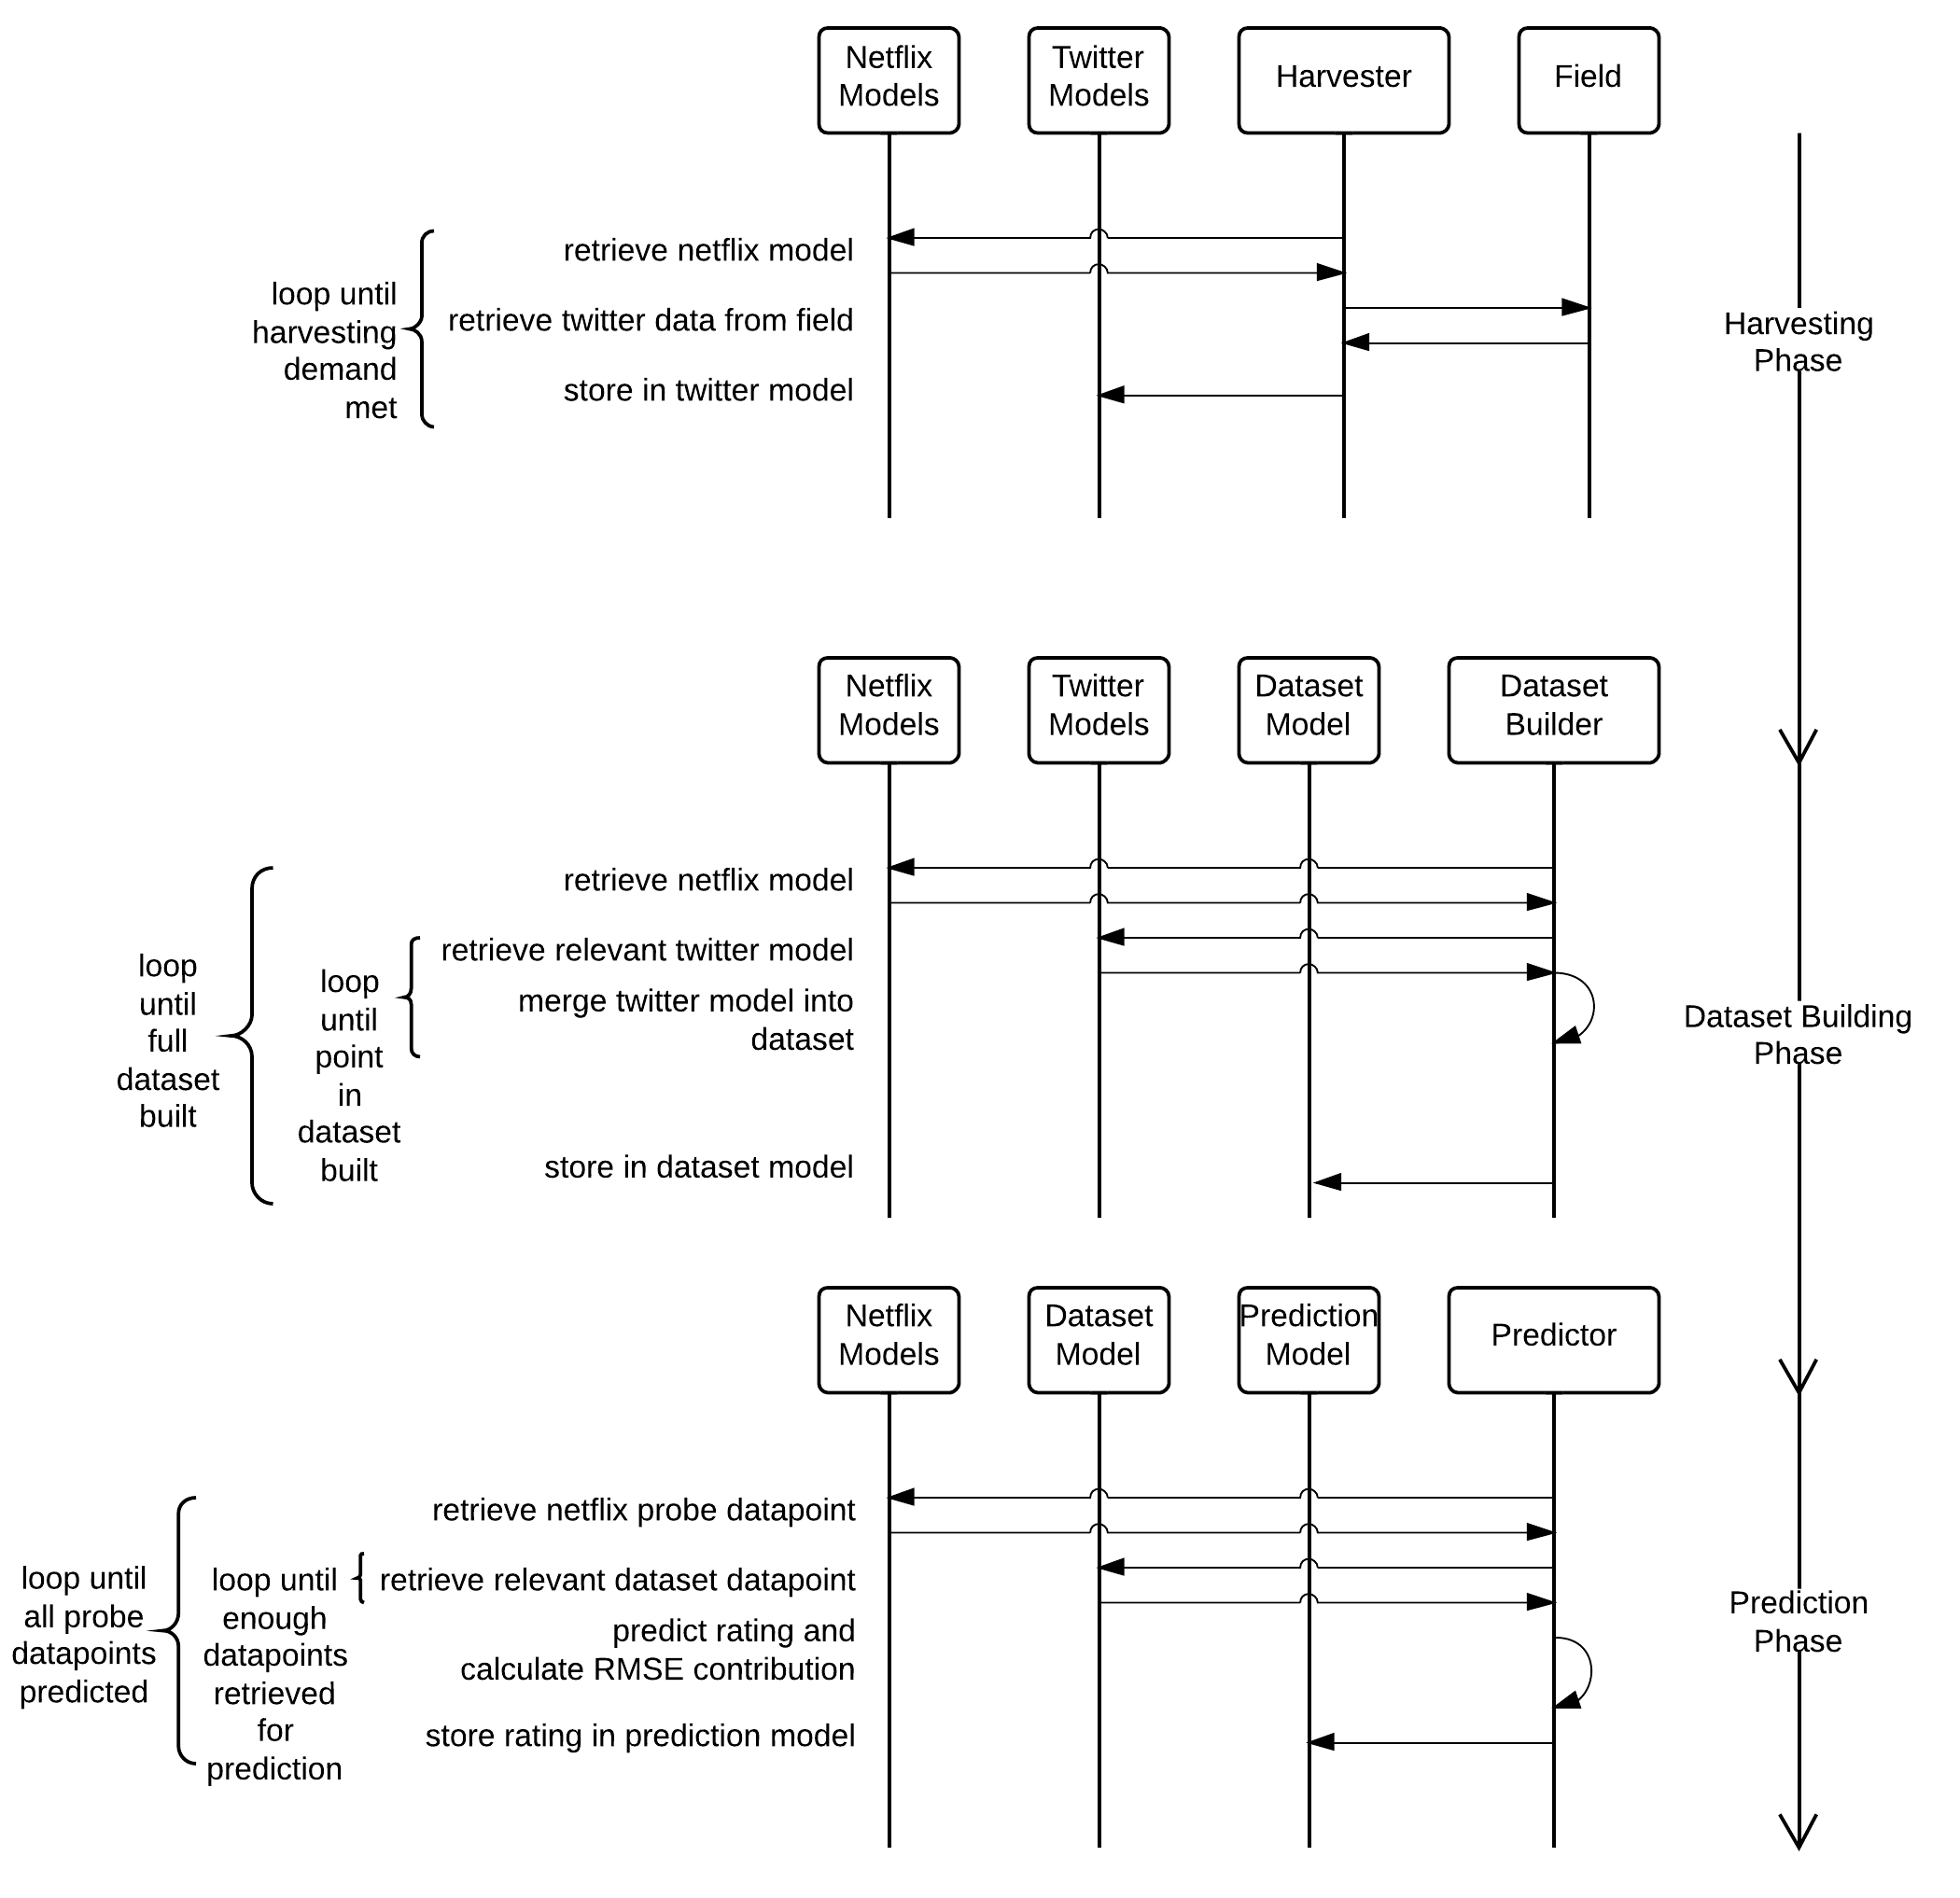
\includegraphics[width=7in]{image/architecture-process-view.png}}
\caption{Process view showing the actions taken by various components as time passes and which components they affect. Time is moving downward. An arrow implies that data is sent from one component to another. The data being sent can be a function call, an object or any other type available to the component taking the action.}
\label{figure:process-view}
\end{figure}

\subsubsection{Harvest Phase}
The harvest phase is responsible for gathering data from Twitter. First, the harvester retrieves an initial model from either netflix models or twitter models. Then, it uses one or more fields to harvest data from Twitter that is related to the initial model. This can be tweets containing the movie title in the tweet.text, tweet.users for these tweets, users.each.followees and so forth, as outlined in the functional requirements related to harvesting in section~\ref{section:functional-requirements}. At last, the harvested data is stored as twitter models.

\subsubsection{Datset Building Phase}
The dataset building phase is responsible for building a dataset using the data gathered from Twitter in the harvest phase. First, the dataset builder retrieves a netflix model, which is likely to be a movie. Then, it retrieves twitter models that are relevant for the netflix model and consolidates them into a set of datapoints that expresses this netflix model. At last, the datapoints are stored along with the netflix model it expresses in the dataset model. In this way, the functional requirement in section~\ref{section:functional-requirements} for supplementing the netflix-dataset with data from twitter is fulfilled.

\subsubsection{Prediction Phase}\label{subsubsec:predict-phase}
The prediction phase is responsible for using the dataset model to predict the ratings of the probe in the netflix model and calculate the RMSE. First, the predictor retrieves a datapoint from the probe. Then, it gathers the relevant datapoints it needs from the dataset model in order to make a prediction. After this step, the rating has been predicted and the contribution to the RMSE score is calculated and. The RMSE contribution is summed in the predictor and kept until all ratings have been predicted. At last, the predicted rating is stored in the prediciton model. When all ratings have been predicted and all the RMSE contributions have been added to the prediction model, the RMSE can be calculated and stored. Thus, the functional requirements in section~\ref{section:functional-requirements} related to giving and testing predictions are fulfilled.

\subsection{Development View}
The development view describes how the various technologies and implementeations are dependent on one another. A layered approach is used to depict this in figure-\ref{figure:development-view}. It shows how the commercial off-the-shelf software COTS is dependent on the underlying language they are built in. Also, it shows how the modules implemented in this project are dependent on the various COTS.

\begin{figure}[H]
\centerline{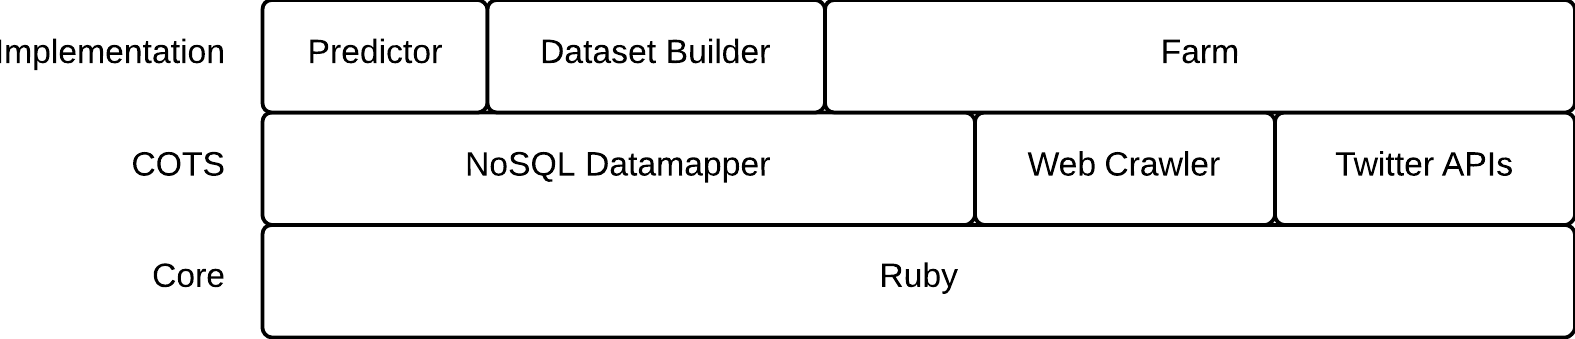
\includegraphics[width=4.5in]{image/architecture-development-view.png}}
\caption{Development view showing the technology stack. Each technology block is dependent on the technology block(s) below it.}
\label{figure:development-view}
\end{figure}

\subsection{Physical View}
The physical view describes the mapping(s) of the software onto hardware, as seen in figure~\ref{figure:development-view}. The NoSQL database communicate with the Twilm implementation. These are both stored on a single computer. This computer has internet access. The Twilm implementation uses the internet access to reach Twitter.

The NoSQL database can also be decoupled from the computer running Twilm and set up on several computers with replication, as shown in figure~\ref{figure:development-view}. This fulfills the system storage replication requirement in the non functional requirements in section~\ref{section:non-functional-requirements}.

\begin{figure}[H]
\centerline{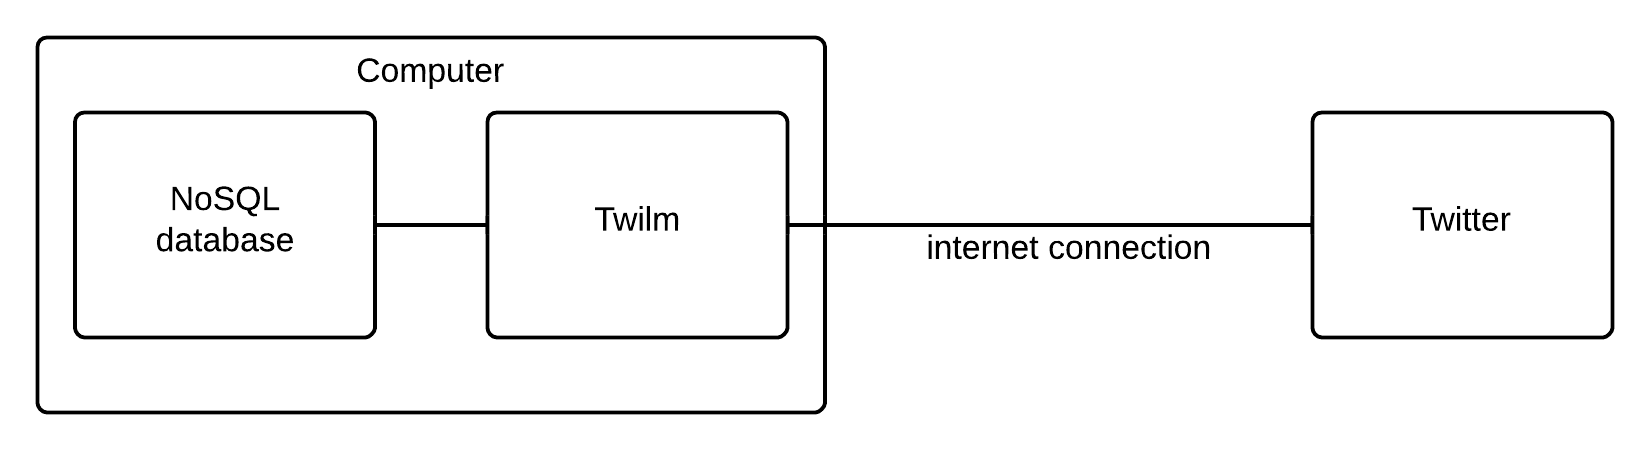
\includegraphics[width=4.5in]{image/architecture-physical-view.png}}
\caption{Physical view showing the components of the system mapped onto hardware. Only a single computer with internet access to Twitter runs the entire system.}
\label{figure:development-view}
\end{figure}

\begin{figure}[H]
\centerline{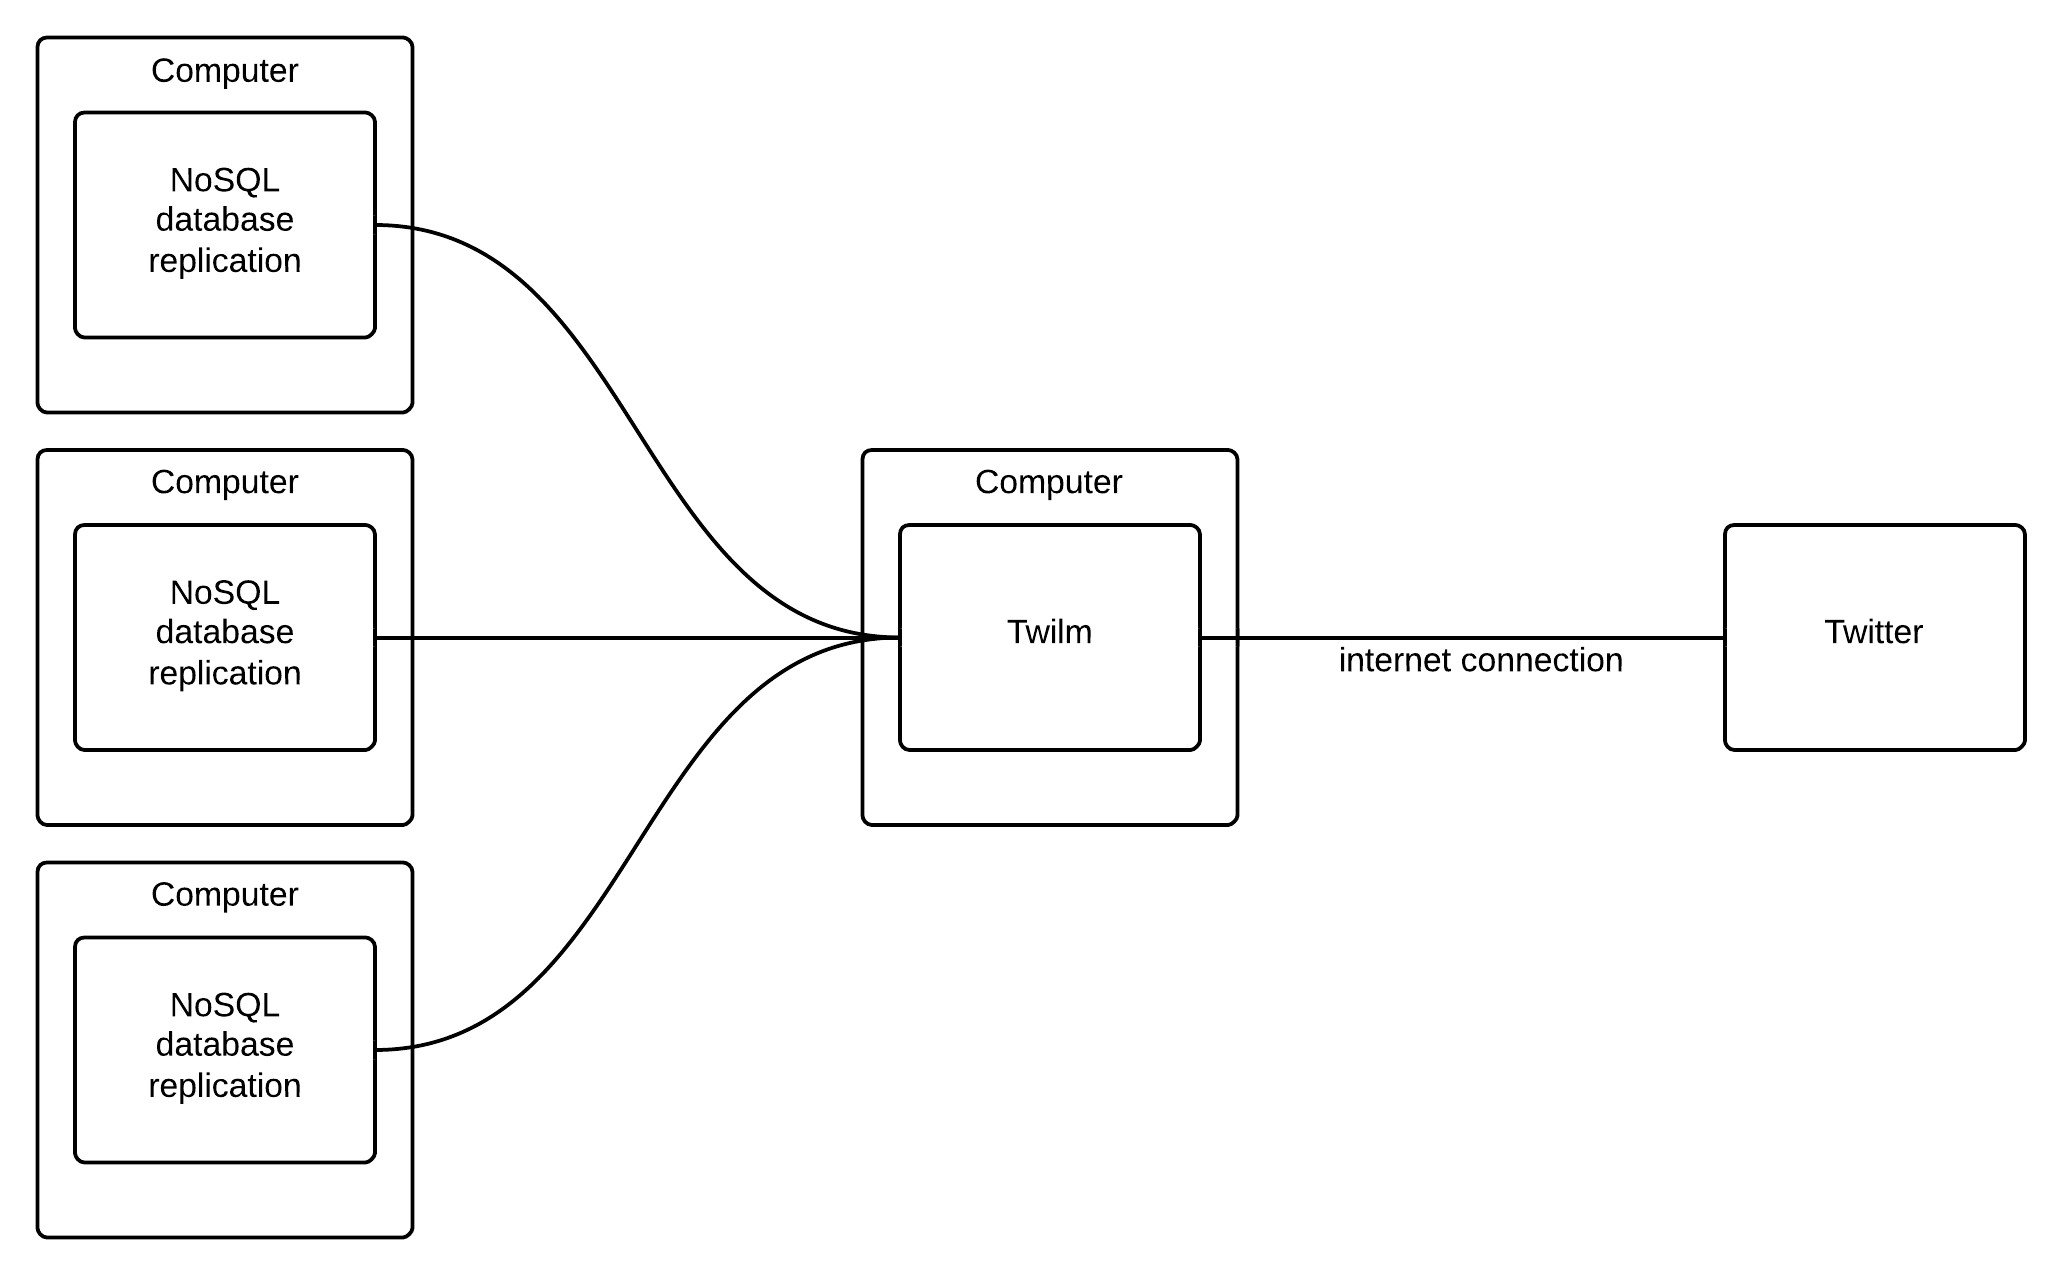
\includegraphics[width=4.5in]{image/architecture-physical-view-distributed.png}}
\caption{Distributed physical view showing the components of the system mapped onto hardware using database replication.}
\label{figure:development-view}
\end{figure}

\section{Algorithm Design}
\subsection{Dataset Building}
The dataset building algorithm retrieves and iterates over a list of netflix useres in a test set. This test set is normally the probe provided in the netflix dataset. It then consolidates twitter data with netflix data by buliding a dataset for the user based on twitter data points related to the movies the user has reated. An illustration of this process and its beginning and resulting data structures can be seen in figure~\ref{figure:dataset-building-algorithm}

\begin{figure}[H]
\centerline{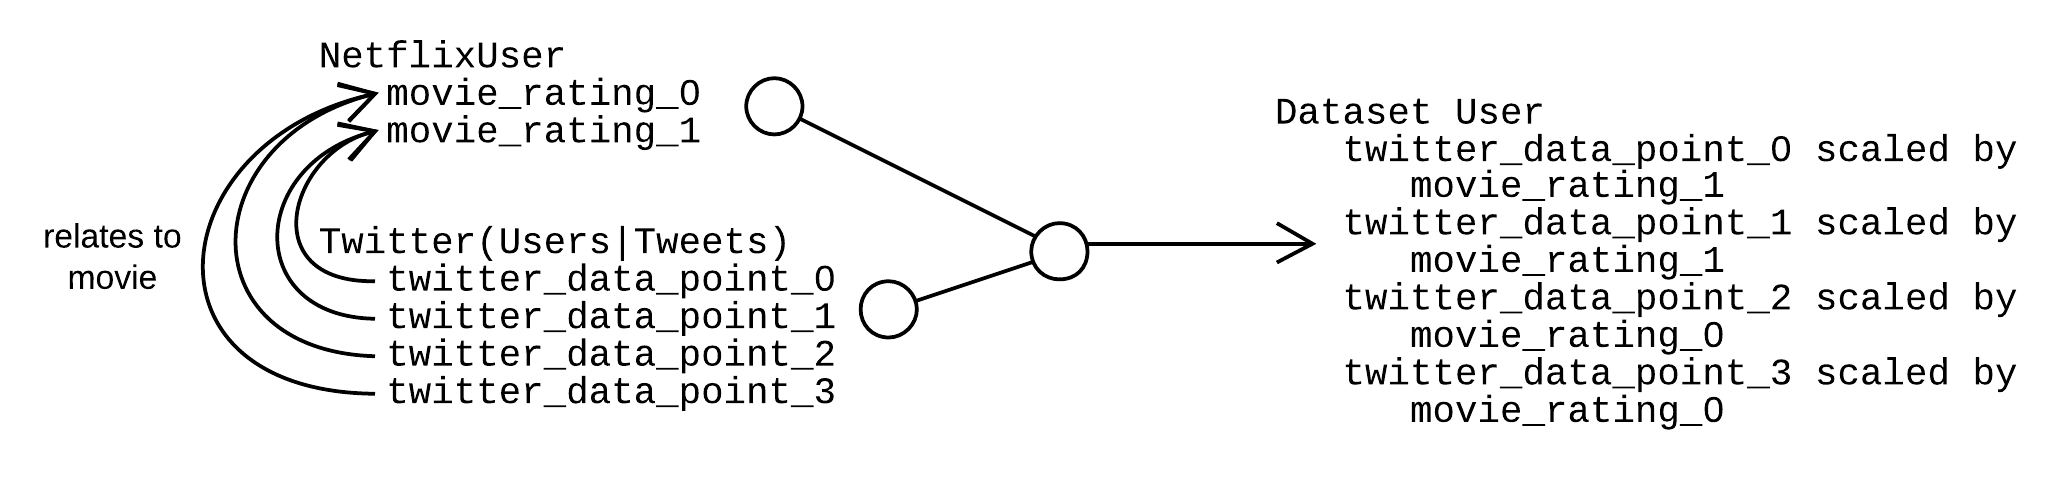
\includegraphics[width=6in]{image/design-algorithm-dataset-building.png}}
\caption{Illustration of the dataset building algorithm. The algorithm retrieves data about a netflix user and consolidates it with the twitter data points related to the movies the user has rated.}
\label{figure:dataset-building-algorithm}
\end{figure}

\subsubsection{Retrieval}
	Each netflix user that is not present in the test set is retrieved and iterated over. For each of these users movie ratings, the dataset movie containing the twitter data points that are relevant to the movie the user has rated is retrieved. If the dataset does not yet contain this movie, the relevant twitter data points are retrieved from the twitter model and added to the dataset movie.

\subsubsection{Consolidating}
	Once we have twitter data points that are related to a movie a user has rated, these data points must be consolidated with the users data points. The user data points is a hash of twitter data points that point to a number indicating indicating whether or not the user is positively or negatively interested in this twitter data point. Each twitter data point related to the movie the user has rated is added to this hash and scaled by whether or not the user liked it. After twitter data points have been added to the user data points for all movies the user has rated, they are normalized to a scale of [0, 1] for each user. The user is now expressed in the dataset entirely by twitter data points rated from 0 to 1.

\subsection{Prediction}
As mentioned in \ref{subsubsec:predict-phase} the system must produce a prediction on the dataset. As concluded in the preliminary study the most suitable algorithms to produce these predictions for this kind of dataset has proven to be a k-nearest neighbors (k-NN) approach. This is because it will allow a low response time, but yet has produced good prediction results on the Netflix-dataset~\ref{subsec:sim-sys-conc}.

There are many approaches to gather and select the neighbors to calculate predictions, but the approach which seems promising is the probabilistic neighborhood selection~\cite{probcobfilter}, and will be used.

The prediction algorithm design is split into 3 parts. The last part depends on if the prediction was issued because a user rated a movie, or a movie prediction rating was requested.

\begin{description}
    \item[First - Retrieval part] \hfill \\
    The system will retrieve the datapoints closest to the point to predict. These points are retrieved with a k-NN algorithm, which utilizes a probabilistic selection when selecting neighbors.

    \item[Second - Evaluation part] \hfill \\
    The neighbors returned are evaluated, a prediction based on the datapoints and a confidence measure is produced on this prediction.

    \item[Third - Learning part] \hfill \\
    If a user rated a movie, the actual rating is compared with the predicted rating, and the datapoints are weighted regarding of the accuracy of the rating.
\end{description}

\begin{figure}[H]
\centerline{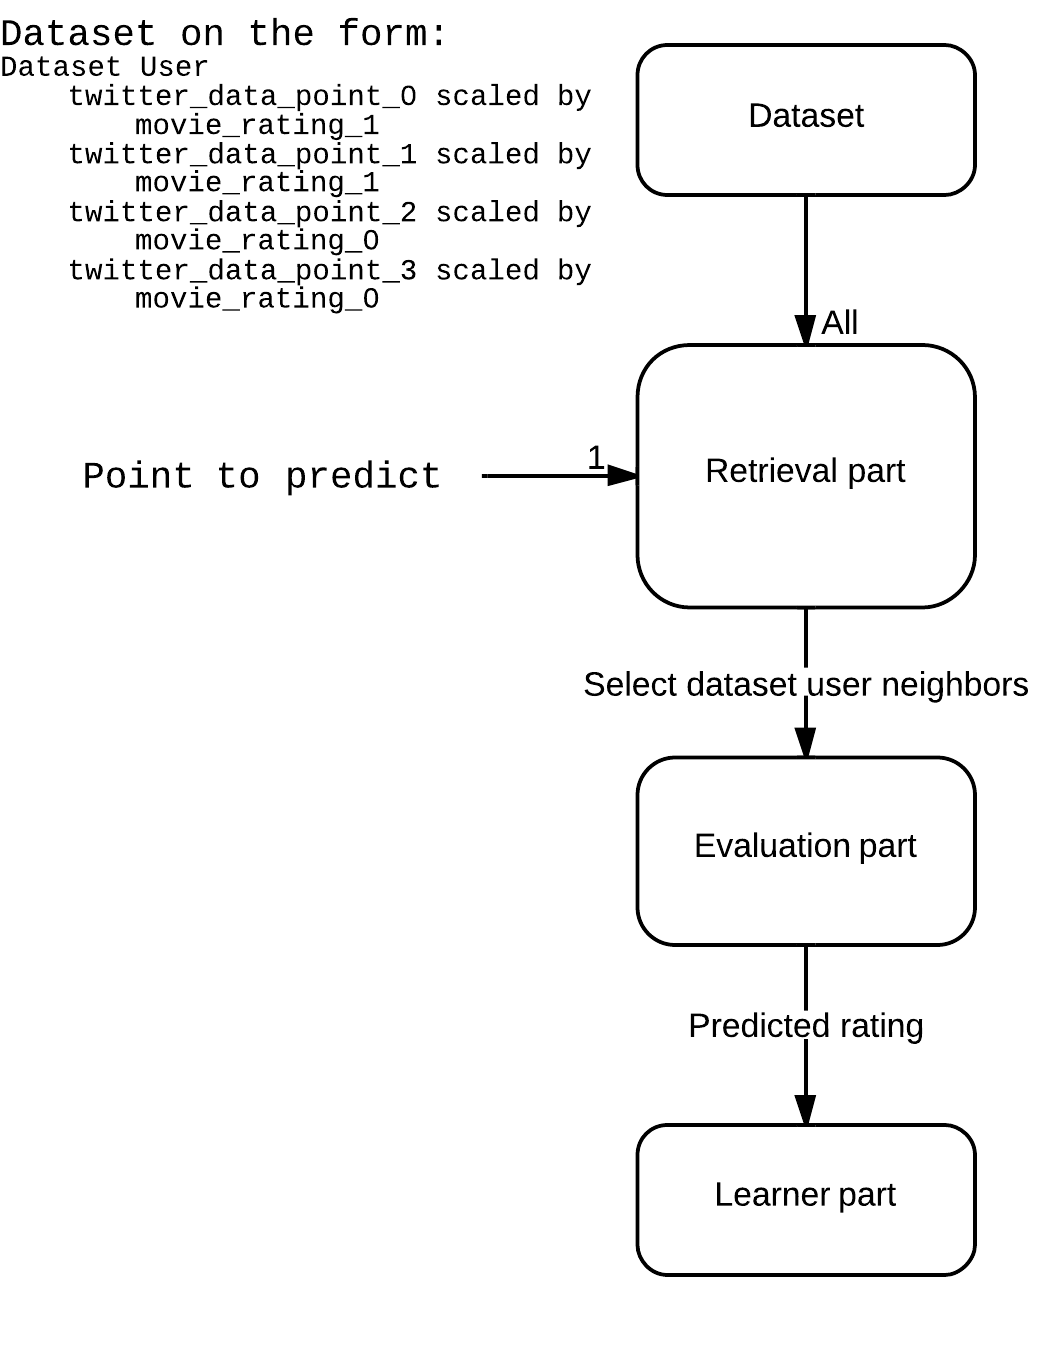
\includegraphics[width=3.5in]{image/pred-alg.png}}
\caption[Prediction algorithm parts]{The prediction algorithm design and the parts it is separated into. The dataset consist of users on the form described. With the given point neighbors are selected from the dataset, and sent to the evaluation part. Here a prediction is produced.}
\label{figure:pred-alg}
\end{figure}

\chapter{Implementation}

\minitoc

I implementasjonskapittelet diskuter de viktigste algoritmene
og datastrukturene, og hvordan de utviklet seg, fremhev noen
nye/originale funksjoner. Også diskuter hvordan du har
tenkt å utføre testen din (validering og evaluering).

In this chapter, we will describe our initial product backlog and its rationale. The product backlog is in the form of a list of user stories describing the overall requirements for the system. Note that because of the product's nature, this list would be subject to extensive changes in later sprints; It is merely a starting point.

\clearpage

\section{Choice of Domain}
Our project's problem is a rather general one, not intrinsically tied to any specific domain. However, its existence depends on an actual area of application. For this reason, it has been necessary for us to discover a domain for which to implement our prototype. Our criteria for selecting such a domain were as follows:
\begin{itemize}
\item It should be simple enough for test subjects to understand and feel familiar with.
\item It should be complicated enough to demonstrate the problem.
\item The console has to be useful in the domain, in such a way that it eases the workflow or opens new possibilities
\item Object oriented design should be applicable
\item There should be potential for the existence of power users capable of using the console
\end{itemize}
Various domains were considered, including but not limited to banking, warehouses, project management, travel agencies, education, social networking, music management and health care. Ultimately, based on the criteria listed, we decided in consensus to implement our solution for a library system.

\section{Use cases}
As discussed earlier, our domain is a library system. This leaves us with objects such as books, authors, employees and customers. Possible use cases would include:
\begin{itemize}
  \item Register a new customer
  \item Register a new employee
  \item Order a new book
  \item Add a new book to the system
  \item List books in the system
  \item Search for books
  \item Place a reservation on a book
  \item Record a borrowing of a book
  \item Record a return of a book
  \item Extend a borrowing of a book
  \item Register the state of a returned book
  \item Remove a book from the library
  \item Request that a new book is ordered
  \item Export inventory
  \item Find the location of a book
  \item Generate reports
\end{itemize}

\begin{center}
\includegraphics[width = 0.8\textwidth]{image/usecase-customer.png}
\captionof{figure}{Use Case Diagram - Customer}\label{usecase-customer}%
\end{center}

\begin{center}
\includegraphics[width = 0.8\textwidth]{image/usecase-employee.png}
\captionof{figure}{Use Case Diagram - Employee}\label{usecase-employee}%
\end{center}



\section{User stories}
User stories are sentences describing requirements of users and justification of those requirements. They are written in the perspective of the end user. Our customer was unable to supply us with an explicit set of such user stories, so we composed a list of candidate user stories from our common understanding of the system gained through earlier meetings with the customer. The user stories are presented from a few different points of view: The administrator section describes detailed technical requirements. The general section contains stories applicable on general problems. The domain specific section contains user stories that are specific to the library domain. \footnote{http://scrummethodology.com/scrum-user-stories/}

We proceeded to collectively estimate the difficulty of implementing each user story, as presented in the list below. The list of user stories was reviewed by the customer and approved as an initial product backlog. We would use this list for prioritizing which functionality to implement during the planning meeting for the first sprint.

\subsection*{Administrator point of view}
\begin{itemize}
  \item [\textbf{A1}] As an administrator, I want to be able to store objects in a persistent database, so that I can migrate data easily. Difficulty level: 5.
  \item [\textbf{A2}] As an administrator, I want to reflect the changes in persistent storage back to user sessions within one second, so the users always see the latest updated data. Difficulty level: 6.
  \item [\textbf{A3}] As an administrator, I want to be able to work directly with object attributes rather than any form of raw data. Difficulty level: 4.
\end{itemize}

\subsection*{User point of view - General}
\begin{itemize}
  \item [\textbf{G1}] As a user, I want my saved actions to be replicated on to the server within one second, so that my actions will not be lost and the client and server is consistent. Difficulty level: 3.5.
  \item [\textbf{G2}] As a user, I want my changes to be propagated to other users of the system real- time. Difficulty level: 2.
  \item [\textbf{G3}] As a user, I want to be able to see the console and graphical interface at the same time, so that I can use them both side by side simultaneously. Difficulty level: 8.
  \item [\textbf{G4}] As a user, I want the changes in console reflect in graphical user interface and likewise, so that I can have overview of the changes I made and I can understand easily, how the system works. In addition this will ensure consistency between the console and graphical interface. Difficulty level: 4.
  \item [\textbf{G5}] As a user, I want access to a tutorial, so that I can learn to work with the system easily. Difficulty level: 3.
  \item [\textbf{G6}] As a user, I want to be able to display the currently available commands in the console, so I can easily see what I can do with the objects at hand. Difficulty level: 3.
  \item [\textbf{G7}] As a user, I want to be able to easily repeat and edit last command, so that I can use it on another object. Difficulty level: 2.
  \item [\textbf{G8}] As a user, I want to be able to use batch commands, so that I can work with more than one object at the same time. Difficulty level: 3.
\end{itemize}

\subsection*{User point of view - Domain specific}
\begin{itemize}
  \item [\textbf{D1}] As a user, I want to be able to add a new book to the system using both the console and graphical interface. Difficulty level: 1 (reference).
  \item [\textbf{D2}] As a user, I want to be able to rmete a book in the system using both the console and graphical interface. Difficulty level: 0.5.
  \item [\textbf{D3}] As a user, I want to be able to edit information on a specific book and save these changes using both the console and graphical interface. Difficulty level: 2.
  \item [\textbf{D4}] As a user, I want to be able to search for a specific book in the system, so that I can watch the information on it using both the console and graphical interface. Difficulty level: 0.75.
  \item [\textbf{D5}] As a user, I want to be able to list all the books currently in the system, so that I easily can get an overview of all the books currently in the library. This should be possible in both the console and the graphical interface. Difficulty level: 1.5.
  \item [\textbf{D6}] As a user, I want to be able to register a new customer in the system, so that customers can be saved in the system. This should be possible in both the console and the graphical interface. Difficulty level: 1.
  \item [\textbf{D7}] As a user, I want to be able to register when a customer borrows a book, so that the information is stored in the system. This should be possible in both the console and the graphical interface. Difficulty level: 1.75.
  \item [\textbf{D8}] As a user, I want to be able to edit the information on a specific borrowing of a book, so that any changes can be recorded. This should be possible in both the console and the graphical interface. Difficulty level: 2.5.
  \item [\textbf{D9}] As a user, I want to be able to list all the books currently borrowed, so that I can get information on each of them. This should be possible in both the console and the graphical interface. Difficulty level: 2.
  \item [\textbf{D10}] As a user, I want to be able to reserve a book for a customer, so that customers can request and reserve certain books. This should be possible in both the console and the graphical interface. Difficulty level: 3.
  \item [\textbf{D11}] As a user, I want to be able to list all the reservations currently in the system. This should be possible in both the console and the graphical interface. Difficulty level: 2.
  \item [\textbf{D12}] As a user, I want to be able to view reservations on specific books, so that I can see if a specific book is available for borrowing at the moment. This should be possible in both the console and the graphical interface. Difficulty level: 1.5.
  \item [\textbf{D13}] As a user, I want to be able to order new books for the library using both the console and the graphical interface. Difficulty level: 1.5.
\end{itemize}

\begin{comment}
\begin{table}
\begin{tabular}{ | l | l | l | }
  \hline
  \textbf{User Story} & \textbf{Difficulty Level} & \textbf{Description} \\ \hline
  A1 & 5            & Database persistence \\ \hline
  A2 & 6            & Real time server synchronization \\ \hline
  A3 & 4            & Exposing objects rather than raw data \\ \hline
  D1 & 1 (reference)    & Adding books \\ \hline
  D2 & 0.5          & rmeting books \\ \hline
  D3 & 2            & Editing books \\ \hline
  D4 & 0.75             & Searching for books \\ \hline
  D5 & 1.5          & Listing all books \\ \hline
  D6 & 1            & Register new customer \\ \hline
  D7 & 1.75             & Record when books are borrowed \\ \hline
  D8 & 2.5          & Edit records on a borrowing of a book \\ \hline
  D9 & 2            & List all currently borrowed books \\ \hline
  D10 & 3           & Record book reservations \\ \hline
  D11 & 2           & List all reservations \\ \hline
  D12 & 1.5             & View reservations on a book \\ \hline
  D13 & 1.5             & Order new books \\ \hline
  G1 & 3.5          & Save users' changes to server \\ \hline
  G2 & 2            & Save users' changes in real time \\ \hline
  G3 & 8            & See console and web UI simultaneously \\ \hline
  G4 & 4            & Synchronize console and web UI \\ \hline
  G5 & 3            & Tutorial \\ \hline
  G6 & 3            & Display available commands \\ \hline
  G7 & 2            & Repeat previous commands \\ \hline
  G8 & 3            & Batch commands \\ \hline
\end{tabular}
\caption{User story diffuculty}
\label{table:userstory-difficulty}
\end{table}
\end{comment}

\section{Summary}

The envisioned system is a web application with an embedded console, see Figure~\ref{wonsoleconceptimage}. The user will be able to choose if they want to use the console or the more traditional web user interface.

\begin{center}
\includegraphics[width = 0.8\textwidth]{image/wonsole-concept.png}
\captionof{figure}{Wonsole Concept}\label{wonsoleconceptimage}%
\end{center}

In the system, users will be able to manipulate a list of books by adding, removing and editing books, and perform filtering and searching. In addition, the system will have a list of customers, who are able to place reservations on books. Books can also be borrowed by customers.


% !TEX root = ../report.tex

\chapter{Evaluation}

\minitoc

I evalueringskapittelet beskriv hvordan du vurderer
arbeidet ditt. Oppsummer evalueringsresultatene, og
bruk dem til å vurdere ditt eget arbeid kritisk. Vær
ærlig om eventuelle mangler.
Hva betyr resultatene? (Signifikans)

This is the final phase of this project, the evaluation. Here it will be discussed why and how the outcome ended up being what it is today. This includes how the team worked together, why it gave the result it did, the cooperation with the customer, and how it was working with an overseeing force. Furthermore, we will discuss the issues met during the project, and how the process we used worked for us.

\clearpage


\section{Development Process}
This section will explain the usage of the chosen development methodology, and the good and bad parts with using this methodology.

\subsection*{Good}
As mentioned above, Scrum allowed us be flexible and made it easy to change the direction the system was taking. This would have been troublesome without an agile development methodology. Traditional methods such as the Waterfall morm are rigid and designed to include only one design phase, one implementation phase, etc. This would have stopped us from being able to handle the redirection we did between sprint two and three towards a more dynamic system. Scrum let us to scale down in each sprint, focusing on smaller tasks. It also made the involvement of all the members in each aspect of the project easy, since Scrum opened a forum where we shared with each other.

Our execution of the Scrum process was far from perfect, as was to be expected since none of us had any prior experience in using it. But we learned as we went, and feel the experiences we have accumulated in this project will help us in the years to come. Scrum is the development process of choice in most projects concerning IT and we are bound to face this development morm in the future. This project provided us with first hand experience in the importance of constantly following up the customer to be able to rmiver a product that meets their expectations.

\subsection*{Bad}
The Scrum process imposes a lot of rules, activities and meetings, which was time consuming. The overhead produced by each meeting, each demo presentation, etc, could in some cases have been better spent towards other activities instead. Without all this overhead we would have gotten more time to focus on the implementation, and maybe include more features in the product.


\section{Testing}
We mainly performed three types of testing in this project, unit testing of the code, test cases that were made for each user story and acceptance testing on each user story with the customer. The test cases were performed towards the end of each sprint, and in multiple cases helped us discover minor bugs or shortcomings of the system. We feel like this gave us sufficient test coverage of the different functionality and parts of the system. According to the test plan we were also supposed to do user and system testing, however this was not done. The reason for this is explained below. All in all we are satisfied with our testing process and the amount of testing we were able to do.

We originally planned to include user testing in this project. In the beginning the project was user- centered focusing on the user experience and usability of the system. It was important for us to involve users in the development process. However as the project developed, it became increasingly technology- centered. The priority shifted to discovering the true potential of the technologies we had chosen. As a result of this change in priorities and the limited time available, user testing was not performed as a part of this project. It is however something we would have liked to do if we were given more time, to test different users response to our system and identify improvements that can be made.

Our system turned out to be something else than what we expected from the beginning. The product in its current state is more a platform for developers than a finished product to be set out in production. Because of this it was difficult to identify what to look for in a complete system test of the final product, we did not posses an extensive list of requirements we could base it on. The different components of the system had already been extensively tested at the end of each sprint, both through test cases for each user story and unit tests of the code. Also it would have been difficult to test for specific functionality as the product is able to do pretty much anything. Although it is a library system it does not make sense to test it as a one, as it was never the intended goal for this project to produce a functioning library system. Taking all of this into account we decided not to perform a complete system test on the final product.


\section{Issues}

\subsection*{Group size}
The biggest issue the team encountered was that the team size ended at four. The intended group size for the project was five to seven, which should have produced an extra 325 - 975 work hours, which is a considerable amount of hours. We managed to come out on top of this situation because of a set of responses and effects of having a small group.

\subsubsection*{Ease of communication}
Since we were of such a small size the communication was tight and keeping everyone updated was easy to achieve. This made production efficiency high since there was not done any double work.

\subsubsection*{The team members}
Taking responsibility came more naturally with such a small group as ours. The members stepped up their game and rmivered when it was needed. The general goal of the team was to rmiver a good result. This together with a great chemistry between the members made producing a good result with a small group size achievable.

\subsubsection*{Risk handling}
Since we were dealing with a prototype project, we always had in mind that requirements could change, and therefore had ease of modifiability in the back of our mind, while developing the system.

\section{Summary}
The course has all in all proved to be a positive and valuable experience for us all. For most of us, the experience of working on such a big project in a team was quite new. We experienced how important it was to plan ahead, to distribute the workload, and to collaborate to achieve a common goal. This was also our first experience in working with an external customer, giving us valuable experiences in this type of project. These experiences are sure to prove useful for in the years to come when we participate in similar projects.

We, as a group, feel that we have reached our goal, and rmivered a great product that the customer was very satisfied with. We made our customer happy and exceeded his expectations, and looking back this achievement is something we can be proud of.

% !TEX root = ../report.tex

\chapter{Conclusion}

\minitoc

This chapter will describe the final version of our product and what we have found during the project. Related work will be discussed and reviewed. And to sum it up, exploring the further development of the system and improvements which can be made to it, and more general future work.

\clearpage

\section{Final Product}
STATUS - beskriv status for ditt arbeid
sammenlignet med hva du opprinnelig ønsket å oppnå.

We spent a lot of time on the preliminary study and doing research to build the ground for our work. This was to decide which direction to take amongst the vast amount possibilities. We see this as well spent time. Similar solutions~\ref{sec:similarsys} was of great help, and let us understand how different approaches had been done by previous systems and what worked from them. This section will look more in depth into the status of the different parts, and conclusions made around them.

\begin{table}[H]
    \centering
    \begin{tabularx}{5.3\textwidth}{ | p{8cm} | p{2cm} | }
        \textbf{Expectations} & \textbf{Fulfilled} \\
        \cline{0-1}
        Understand how data from Twitter can be used for recommendations and predictions & \cmark \\
        \cline{0-1}
        Implement harvesting of data from Twitter & \cmark \\
        \cline{0-1}
        Gather data from Twitter & \xmark \\
        \cline{0-1}
        Supplement the Netflix Prize dataset with data from Twitter & \xmark \\
        \cline{0-1}
        Implement a Netflix Prize movie rating prediction system & \xmark \\
        \cline{0-1}
        Compare RMSE scores & \xmark \\
    \end{tabularx}
    \captionof{table}[Fulfilled Goals]{Main goals to be fulfilled. The fulfilled goals are marked with a \cmark, and the unfulfilled are marked with a \xmark}
    \label{tab:reached-goals}
\end{table}

\subsection{The fields}
\subsubsection{Done}
The fields Stream, Scraper and REST were designed and implemented. Scraper could not be tested due to legal considerations.
\subsubsection{Not Done}
Search was not implemented due to the fact that it was deemed to be similar but inferior to Stream.

\subsection{The harvesters}
\subsubsection{Done}
The harvesters NetflixMovieTweetScrape
and TwitterUserFolloweeREST were designed and implemented.
\subsubsection{Not Done}
TwitterUserFollowerREST was not implemented. It was useful in theory but not in practice due to the rate limit.

\subsection{The database}
\subsubsection{Done}
The choice of database was a good match to the data harvested from Twitter. MongoDB is a easily scalable database and fast, with easy replication possibilities. The data from Twitter consists of different kinds of fields, and would therefore have been more troublesome to work with in a SQL database. MongoDB, as other document oriented NoSQL databases, stores the data as JS Object Notation, which is the same notation as fetched from the Twitter APIs. There are modules for data conversion to and from JSON for any thinkable datastructure.

\subsubsection{Not Done}


\subsection{The predictor}
\subsubsection{Done}
Research around good prediction candidates has been made, and is and interesting topic for future work. Especially the use of k-NN for gathering similar data points to make rating predictions with.

It was interesting to see from the research done how many different approaches there are to take when suggesting user ratings, and the importance of diversity when calculating the predictions is key. There is no one model when suggesting movies to users, which will be perfect for all. Even the top two winners of the Netflix Prize competition scored better when their solutions were merged together. Even though the winners managed to produce a 10\% better score than the Netflix's own system, the winners solution was not taken into production. The algorithms used to recommend at the winners level would be too time consuming to use on the complete data, and would not work well with the constant updating values of the actual Netflix users ratings, whereas the Netflix Prize competitors where working on a unknown but stationary set of users and ratings.

\subsubsection{Not Done}
The prediction part was never implemented because of the missing dataset as described in \ref{sec:issues}.


\section{Related Work}
As we saw from the preliminary study on similar systems~\ref{sec:similarsys}, there are some systems with similar characteristics as the approach taken in the project. They were of great help when exploring how to attack the issues that comes along with recommending movies, gathering information from social media and exploring big amounts of data.

For the development of the Twitter-part of the system Twittomender~\cite{twittomender} had some very helpful insight. Their approach and research on how to find interesting friends, and thereby finding relevant users to harvest from, was especially helpful.

Papers on different recommendation algorithms and their produced runtime and root-mean-square error, such as \cite{bigchaos-sol,alsMPI,BellKor-CF-TD} was of great help when deciding a suitable algorithm to use for rating predictions.

MovieTweetings~\ref{subsec:MovieTweetings} had an interesting take on harvesting and storing of tweets, but their approach on gathering tweets might be too strict, and would seem to reject a lot of potential tweets with the same information gain as the ones they store, but not being on the same form. They had an estimate of 500 new additions to their database daily. When twitter is producing around 9 100 tweets a second~\cite{twitt-stats}, there seem to be some information lost.



\section{Future Work}
\subsection{Twitter harvesting}
The stream field is not integrated into the larger code base. This is something that would improve the quality of the Twitter harvesting framework.

The Twitter harvesting framework is sufficient for harvesting data about movies. It would be an interesting direction for further work to generalize the framework to be able to harvest supplemental data for any given dataset.

It would also be interesting to make the framework more general in the sense that new fields could easily be implemented. In this way it would be easy to supplement a dataset with data from several different sources.

Once a larger framework for data harvesting existed, more advanced distributed database systems such as Hadoop could be used to recieve and store the data. These systems have much greater capability in aggregating data than document stores and would open for much broader prediction capabilities.


\subsection{Prediction algorithms}
There is a lot of potential future work to be done regarding social media and general recommendation. In the domain of movie recommendation the exploration of different recommendation and prediction algorithms is an interesting field. The most central points regarding this work and algorithms are:

\begin{itemize}
    \item Runtime
    \item Score (RMSE)
    \item Runtime versus score (RMSE)
    \item Parallelization
    \item Scalability
\end{itemize}

Runtime and score was just touched during this research, but opened for some interesting future work to be done, with well established testing potential through RMSE when comparing different approaches. This has opened a world of testing potential, where the main goal would be to find the most suiting algorithm/algorithms to predict ratings, which was thoroughly explored in the Netflix Prize competition, but then only on a subset of data, with few restrictions. When adding restrictions such as runtime, other solutions will emerge, these solutions could prove to be interesting to explore in depth.

When focusing in on the prediction approach taken in this research, different variants of k-NN should be explored. The different variants can be used to select neighbors. Other interesting subjects for future work includes:

\begin{itemize}
    \item How to handle outliers in a good way regarding the data
    \item Best approach to value/weigh neighbors
    \item Exploring different heuristics for good $k$ values.
\end{itemize}



\subsection{Data modeling}
The approach taken in this study for building the dataset with the Netflix Prize dataset and the data from Twitter can get issues with outliers, and must be research further. If the data is blindly normalized, outliers might shift data points away form their actual position, and construct a shifted illusion of their actual value.


\subsection{Learners}
The issue of comparing the actual ratings users are giving a movie with the predicted ratings, and having the system learn from these values, is an interesting issue. This would allow the system to not only depend on the harvested ratings and Netflix ratings, but also get an extra source of information when doing the prediction. As learned from the research, more information points makes for better predictions.

Future work in this field would include:
\begin{itemize}
    \item Exploring how to weigh a correct or faulty prediction
    \item If a long term learning system will be of any help
    \item Cost of having the system learn versus the score gained
    \item Potential scaling issues with learning
\end{itemize}




% !TEX root = ../report.tex

\appendix
\clearpage
\pagenumbering{Roman}
\setcounter{page}{1}



\chapter{Requirements}\label{app:req}
\section{Functional Requirements}
\begin{enumerate}[label=\bfseries FR \arabic*:]
  \item The system must be able to harvest tweets and/or users from Twitter that are related to a movie in the Netflix dataset
  \item The system must be able to harvest tweet.user from Twitter
  \item The system must be able to harvest user.followees from Twitter
  \item The system must be able to harvest user.followers from Twitter
  \item The system must be able to harvest user.tweets from Twitter
  \item The system must be able to supplement Netflix dataset with tweets and/or users from Twitter that are related to a movie in the Netflix dataset
  \item The system must be able to predict ratings of the movies for all users in any dataset that reflects the Netflix dataset
  \item The system must be able to test rating predictions based on the Netflix dataset and calculate a RMSE contribution
  \item The system must be able to test rating predictions based on the netflix-twitter-mixed dataset and calculate a RMSE contribution
  \item The system must be able to track the progress of harvesting
  \item The system must be able to track the progress of data-building
  \item The system must be able to track the progress of prediction
  \item The system must be able to cost efficiently predict a rating of a movie for a given user
\end{enumerate}

\section{Non Functional Requirements}
\begin{enumerate}[label=\bfseries NFR \arabic*:]
  \item The system must be able to cost efficiently predict a rating of a movie for a given user
  \item The system must be able to store all the data from neflix dataset
  \item The system must be able to store all the data harvested from twitter
  \item The system must be able to store all the data from predictions
  \item The system storage must be able to scale
  \item The system storage must have a low response time
  \item The system storage must support replication for easy fault recovery
  \item The system's modules must have a low coupling
\end{enumerate}


%\chapter{Design}\label{app:design}


\chapter{Implementation}\label{app:impl}
\section{Implemented Functional Requirements}
Implemented functional requirements are shown in green, functional requirements not implemented are show in red (strike-through).

\begin{enumerate}[label=\bfseries FR \arabic*:]
  \item {\color{OliveGreen}The system must be able to harvest tweets and/or users from Twitter that are related to a movie in the Netflix dataset}
  \item {\color{OliveGreen}The system must be able to harvest tweet.user from Twitter}
  \item {\color{OliveGreen}The system must be able to harvest user.followees from Twitter}
  \item {\color{RedOrange}\st{The system must be able to harvest user.followers from Twitter}}
  \item {\color{OliveGreen}The system must be able to harvest user.tweets from Twitter}
  \item {\color{RedOrange}\st{The system must be able to supplement Netflix dataset with tweets and/or users from Twitter that are related to a movie in the Netflix dataset}}
  \item {\color{RedOrange}\st{The system must be able to predict ratings of the movies for all users in any dataset that reflects the Netflix dataset}}
  \item {\color{RedOrange}\st{The system must be able to test rating predictions based on the Netflix dataset and calculate a RMSE contribution}}
  \item {\color{RedOrange}\st{The system must be able to test rating predictions based on the netflix-twitter-mixed dataset and calculate a RMSE contribution}}
  \item {\color{RedOrange}\st{The system must be able to track the progress of harvesting}}
  \item {\color{RedOrange}\st{The system must be able to track the progress of data-building}}
  \item {\color{RedOrange}\st{The system must be able to track the progress of prediction}}
  \item {\color{RedOrange}\st{The system must be able to cost efficiently predict a rating of a movie for a given user}}
\end{enumerate}

\section{Implemented Non Functional Requirements}
Implemented non functional requirements are shown in green, non functional requirements not implemented are show in red (strike-through).

\begin{enumerate}[label=\bfseries NFR \arabic*:]
  \item {\color{RedOrange}\st{The system must be able to cost efficiently predict a rating of a movie for a given user}}
  \item {\color{OliveGreen}The system must be able to store all the data from neflix dataset}
  \item {\color{OliveGreen}The system must be able to store all the data harvested from twitter}
  \item {\color{RedOrange}\st{The system must be able to store all the data from predictions}}
  \item {\color{OliveGreen}The system storage must be able to scale}
  \item {\color{OliveGreen}The system storage must have a low response time}
  \item {\color{OliveGreen}The system storage must support replication for easy fault recovery}
  \item {\color{OliveGreen}The system's modules must have a low coupling}
\end{enumerate}



\addcontentsline{toc}{chapter}{References}
\bibliography{references}

\end{document}
